% -------------------------------------------------------------------------------
% 
\documentclass[10pt,xcolor=svgnames]{beamer}
%\documentclass[10pt,draft,xcolor=svgnames]{beamer}

% -------------------------------------------------------------------------------

%% Include only:

%\includeonly{content/01_intro}
%\includeonly{content/02_data}
%\includeonly{content/03_toy_model}
%\includeonly{content/04_interpret}
%\includeonly{content/05_apps,content/06_conclu}
%\includeonly{content/0A_bonus}

% Title page and bibliography are in this file. 
% Sections and bonus material are in ./content/ .
% Macros are in ./pres_macros.tex and font options in pres_font.sty
% -------------------------------------------------------------------------------

%% Packages, beamer style and macros files

% To refer to section name
\usepackage{nameref}

% Bibliography style, add title on bibliography page
\usepackage[round]{natbib}

% ** if draft
\usepackage{ifdraft}

% Import graphical package (add path to figures and diagrams)
\usepackage{graphicx}
\graphicspath{{figures/eps/}{figures/diagrams/}{figures/crop/}}

% Tikz for diagrams and annotation
\usepackage{tikz}
\usetikzlibrary{arrows,calc,decorations.pathmorphing,shapes,trees}
\tikzstyle{every picture}+=[remember picture]
\usetikzlibrary{positioning}
\usepackage{wasysym}          % additional characters

% Import mathematical packages (equation numbering by section)
\usepackage{amsmath,amsfonts,amssymb}  
%\numberwithin{equation}{section}

%	Import beamer style in ./beamerthemeepres.sty 
% (includes the \mytitlepage and \tikzfig commands}
\usetheme{pres}

% Import macros in ./pres_macro.tex
% 
% pres_macros.tex
%
% LaTeX macros and shortcuts for my MS presentation
%
% -----------------------------------------------------------------------------

\usepackage{color}		
\usepackage{xspace}
\usepackage{amsfonts,amssymb,nicefrac}
\usepackage{xargs}

%% Text shortcuts 

% Presentation acronyms
\newcommand{\coeffs}{coeffs.\xspace}
\newcommand{\tmcoeffs}{toy model coeffs.\xspace}
	
% Common abbreviations 
\newcommand{\ie}{i.e.\xspace }
\newcommand{\eg}{e.g.\xspace }
\newcommand{\etc}{etc. \@\xspace}
\newcommand{\esp}{esp.\xspace}
\newcommand{\wrt}{w.r.t.\xspace}
\newcommand{\vs}{vs.\xspace}

% Dataset names
\newcommand{\ccsm}{CCSM 3.0\xspace}
\newcommand{\hadgem}{HadGEM1\xspace}
\newcommand{\era}{ERA-40\xspace}
\newcommand{\ncep}{NCEP-DOE\xspace}

% Common subscripts
\newcommand{\tm}{\subt{TM}}

% Model variables
\newcommand{\mrso}{mrso\xspace}
\newcommand{\mrsos}{mrsos\xspace}

% Common chemical formulae
\newcommand{\COtwo}{$\text{CO}_\text{2}$\xspace}

% 20th, 21st century
\newcommand{\twentyth}{20th\xspace}
\newcommand{\twentyfirst}{21st\xspace}
% -----------------------------------------------------------------------------

%% Math macros and shortcuts

% 1 point space command (before and after brackets)
\newcommand{\pt}{\hskip1pt}

% custom side fractions
\newcommand{\Nfrac}[2]{\raisebox{0.3ex}{$#1$}\big/\raisebox{-0.3ex}{$#2$}}

% inverse
\newcommand{\inv}{^{-1}}
\newcommand{\invv}{^{-2}}

% side fractions
\newcommand{\half}{{\nicefrac{1}{2}}}

% improved over-bar and inner product
\newcommand{\barr}[2][{}]{\overline{\!#2\,}^{#1}} 
\newcommand{\innerp}[2]{\big\langle\pt#1,#2\pt\big\rangle}

% statistical operators
\DeclareMathOperator{\Var}{Var}
\DeclareMathOperator{\Cov}{Cov}
\DeclareMathOperator{\corr}{corr}
\DeclareMathOperator*{\Corr}{Corr}
\DeclareMathOperator*{\proj}{Proj}

% error operator
\DeclareMathOperator*{\Err}{Err}
\DeclareMathOperator*{\rms}{RMS}

% sign operator
\DeclareMathOperator*{\sgn}{sign}

% calculus operators
\newcommand{\derv}[2]{\frac{\mathrm{d}\hskip1pt{#1}}{\mathrm{d}\hskip0.5pt{#2}}}
\newcommand{\dervside}[2]{\nicefrac{\mathrm{d}{#1}}{\mathrm{d}{#2}}}

% subscripts in italic text
\newcommand{\subt}[1]{_{\mathit{#1}}}

% time increment
\newcommand{\Deltat}{{\Delta\!t}}

% imply and if and only if symbols (with spacing as optional argument)
\renewcommandx*{\iff}[1][1={}]{{#1}\Longleftrightarrow{#1}}
% -------------------------------------------------------------------------------

%% Symbols shortcuts

% toy model expression for T' , Var(T) and m' , Var(m)
\newcommand{\Ttm}{\hat{\!T\,}_\mathit{\hskip-0.65ex tm}'}
\newcommand{\VarTtm}{\Var(\hat{\!T\,}_\mathit{\hskip-0.65ex tm})}
\newcommand{\mtm}{\hat{\hskip-0.5pt m\,}_\mathit{\hskip-0.25ex tm}'}
\newcommand{\Varmtm}{\Var(\hat{\hskip-0.5pt m\,}_\mathit{\hskip-0.25ex tm})}

% radiation forcing (with same subscript size)
\newcommand{\Fsw}{F_{\raisebox{-0.3ex}{$\scriptstyle{\mathit{sw}}$}}}
\newcommand{\Flw}{F_{\scriptstyle{\mathit{lw}}}}

% up / down arrows
\newcommand{\up}{^{\,\,\uparrow}}
\newcommand{\upp}{^{\,\,\uparrow'}}
\newcommand{\down}{^{\,\,\downarrow}}
\newcommand{\downn}{^{\,\,\downarrow'}}

% bar averages shortcuts
\newcommand{\Tbar}{\barr{T}}
\newcommand{\mbar}{\barr{m\hskip-1pt}}
\newcommand{\Fbar}{\barr{F}}
\newcommand{\Ebar}{\barr{E}}
\newcommand{\Hsbar}{\barr{H_s}}
\newcommand{\Flubar}{\barr{\Flu}}
\newcommand{\Pbar}{\barr{P}}
\newcommand{\Rbar}{\barr{R}}
\newcommand{\mbbar}{\barr{m_b}}
\newcommand{\Xbar}{\barr{X}}

% longwave up term (full, anomaly, anomaly param. residual)
\newcommand{\Flu}{{F_{\scriptscriptstyle{\mathit{lw}}}
											^{\scriptscriptstyle\,\,\uparrow}}}
\newcommand{\Fluu}{F_{\scriptscriptstyle{\mathit{lw}}}
											^{\scriptscriptstyle\,\,\uparrow\,'}}
\newcommand{\Fluuo}{F_{\scriptscriptstyle{\mathit{lw}0}}
											^{\scriptscriptstyle\,\,\uparrow\,'}}

% sensible heat term (anomaly param. residuals)
\newcommand{\Hso}{H_{\raisebox{3pt}{$\scriptstyle\hskip-1pt s \hskip0.5pt 0$}}'}
\newcommand{\HsO}{H_{\raisebox{3pt}{$\scriptstyle\hskip-1pt s \hskip0.5pt 0$}}}
\newcommand{\Hsoo}{H_{\raisebox{3pt}{$\scriptstyle\hskip-1pt s \hskip0.5pt 00$}}'}

% skin temperature
\newcommand{\Tsk}{T\subt{skin}}

% budget residuals
\newcommand{\xiU}{\xi_U}
\newcommand{\xiUbar}{\barr{\xi_U}}
\newcommand{\xim}{\xi_m}
\newcommand{\ximbar}{\barr{\xi_m}}

% toy model coefficients
\newcommand{\nuE}{\nu_{\scalebox{0.7}{$\hskip-1pt E$}}}
\newcommand{\nuHs}{\nu_{\scalebox{0.7}{$\hskip-1.5pt H\hskip-1pt s$}}}
\newcommand{\nuI}{\nu_{\scalebox{0.7}{$\hskip-1pt I$}}}
\newcommand{\nus}{\nu_{\hskip-1pt s}}
\newcommand{\gammaHs}{\gamma_{\scalebox{0.7}{$\hskip-2.5pt H\hskip-1pt s$}}}
\newcommand{\gammalw}{\gamma_{\scalebox{0.7}{$\hskip-2.5pt l\hskip-1pt w$}}}
\newcommand{\gammaG}{\gamma_{\scalebox{0.7}{$\hskip-1.5pt G$}}}

% alternative toy model coefficients and residuals 
\newcommand{\nuHsalt}{\tilde{\nu_{\scalebox{0.7}{$\hskip-1.5pt H\hskip-1pt s$}}}}
\newcommand{\gammaalt}{\tilde{\gamma}\;}
\newcommand{\chialt}{\tilde{\chi}\;}
% -----------------------------------------------------------------------------

%% Units shortcuts

% time
\newcommandx*{\s}[1][1={}]{\,\ensuremath{\text{s}^{#1}}\xspace}
\newcommandx*{\Day}[1][1={}]{\,\ensuremath{\text{day}^{#1}}\xspace}

% length
\newcommandx*{\m}[1][1={}]{\,\ensuremath{\text{m}^{#1}}\xspace}
\newcommandx*{\mm}[1][1={}]{\,\ensuremath{\text{mm}^{#1}}\xspace}
\newcommandx*{\cm}[1][1={}]{\,\ensuremath{\text{cm}^{#1}}\xspace}

% mass
\newcommandx*{\kg}[1][1={}]{\,\ensuremath{\text{kg}^{#1}}\xspace}

% temperature
\newcommandx*{\K}[1][1={}]{\,\ensuremath{\text{K}^{#1}}\xspace}
\newcommand{\degC}{\,\ensuremath{^\circ\text{C}}\xspace}

% Energy
\newcommandx*{\J}[1][1={}]{\,\ensuremath{\text{J}^{#1}}\xspace}
\newcommandx*{\W}[1][1={}]{\,\ensuremath{\text{W}^{#1}}\xspace}
\newcommandx*{\Wm}[1][1={}]{\,\ensuremath{\text{Wm}^{#1}}\xspace}

% Pressure
\newcommandx*{\Pa}[1][1={}]{\,\ensuremath{\text{Pa}^{#1}}\xspace}
% -----------------------------------------------------------------------------

%% Environments

% A nicer-looking cases environment (easier to code as a command ...)
\newcommand{\nicecases}[5]{\begin{cases}
		\;\;#1 \\ \;\;#4 \end{cases}
		\text{#2}
		\quad \vspace*{-1em}
		\begin{array}{l}#3 \\ #5\;.\end{array}}  

% A variant ... Using & to align #2
\newcommand{\Nicecases}[5]{\begin{cases}
		\;\;#1 \\ \;\;#4 \end{cases}
		\mbump\mbump&\text{#2}
		\quad \vspace*{-1em}
		\begin{array}{l}#3 \\ #5\end{array}}  
	
% -----------------------------------------------------------------------------
    

% Font choices and adjustments in ./pres_font.sty
\usepackage{pres_font}          
\DeclareMathSizes{10}{11.5}{8}{7}

% Math environment formating
\AtBeginDocument{\setlength{\abovedisplayskip}{1em}}
%\AtBeginDocument{\setlength{\abovedisplayshortskip}{0em}}
%\AtBeginDocument{\setlength{\belowdisplayskip}{0.75em}}	
%\AtBeginDocument{\setlength{\belowdisplayshortskip}{1em}}	
%\AtBeginDocument{\setlength{\jot}{0.5em}}		% in-between rows in align

% -------------------------------------------------------------------------------

%% Definitions 

% Title
\title[]%
{Linking Soil Moisture \\ {\Large and} \\ 
 Summertime \\ Surface Temperature Variability}

% Authors
\author[]%
{\'Etienne T\'etreault-Pinard 
 \\[1em] {\small David Battisti}   
 \\ {\small Abby Swann, Dargan Frierson, Marcia Baker}   
}
% \\[0.7em] {\small Committee members: A} 

% Date 
\date[]%
{October 24, 2013}

% ------------------------------------------------------------------------------- 

\begin{document}
 
%% Title page
\mytitlepage

% -------------------------------------------------------------------------------

%% Content

%
% Section 1: Introduction
%
%   # of slides: 10
%
% -------------------------------------------------------------------------------
\section{Introduction}
\label{sec:intro}

\begin{frame}
\frametitle{Why Study Temperature Variability?}

\begin{itemize}

\item {Recent summertime heat waves / droughts:}

\end{itemize}

\begin{center}

\tikzfig{intro_fig}{width=0.75\linewidth}

\end{center}

\begin{tikzpicture}[overlay]

\coordinate (p2003) at ($(intro_fig.west)+(1.75,0.5)$);
\coordinate (p2010) at ($(intro_fig.west)+(-0.5,-2)$);
\coordinate (p2012) at ($(intro_fig.east)+(0.5,-2)$);

\node[color=colone,font=\bf] at (p2003) {2003};
\node[color=colone,font=\bf] at (p2010) {2010};
\node[color=colone,font=\bf] at (p2012) {2012};

\end{tikzpicture}

\end{frame}

\begin{frame}
\frametitle{Temperature variability projections}

\begin{columns}

  \begin{column}{0.35\linewidth}

  \vspace*{-2em}
  \begin{itemize}

  \item \citet{schar04}: \textcolorbf{coltwo}{increasing \COtwo} could lead to
  \textcolorbf{coltwo}{increasing summertime $T$ variability} in some locations.

  \item \textcolorbf{colone}{Left panel:} \newline \vspace*{-1em}
  $\barr{T}_{2071-2100}-\barr{T}_{1961-1990}$ \\[1.5em]

  \textcolorbf{colone}{Right panel:} \newline \vspace*{-0.5em}
  $\dfrac{\sigma_{\!T,2071-2100}-\sigma_{\!T,1961-1990}}{\sigma_{\!T,1961-1990}}$ 

  \end{itemize}

  \end{column}
  
  \begin{column}{0.6\linewidth}

  \vspace*{-0.6em}
  \hspace*{0.7em}
  \tikzfig{schar04_map}{trim=0cm 2.4cm 0.1cm 0cm,clip,width=0.98\linewidth}

%  \vspace*{-1.8em}
%  \tikzfig{schar04_pdf}{trim=0cm 0cm 0.1cm 0cm,clip,width=\linewidth}

  \end{column}

\end{columns}

\end{frame}

\begin{frame}
\frametitle{Role of soil moisture / {\normalsize land-atmosphere interactions}}

\vspace*{-2.5cm}
\begin{itemize}

\item \citet{sene06_coupling}: 4 GCM simulations:

\end{itemize}

\begin{center}

\tikzfig{sene06_sig_T}{trim=0cm 0.4cm 7.5cm 0cm,clip,width=0.68\linewidth}

\vspace*{-4cm} 
\tikzitemMark
\end{center}

\begin{tikzpicture}[overlay]

\coordinate (title) at ($(sene06_sig_T.north)+(0,-0.1)$);
\coordinate (units) at ($(sene06_sig_T.east)+(0.3,-1.7)$);
\coordinate (label1) at ($(sene06_sig_T.west)+(-0.5,2)$);
\coordinate (label2) at ($(sene06_sig_T.west)+(-0.5,-1)$);
\coordinate (label3) at ($(sene06_sig_T.south)+(-1.8,-0.1)$);
\coordinate (label4) at ($(sene06_sig_T.south)+(1.8,-0.1)$);

\node[color=colone,font=\bf] at (title) {Standard deviation of $T$ (JJA)};
\node at (units) {[$\degC$]};
\node[color=colone,align=left,font={\small \bf}] at (label1) 
  {evolving \\ soil moisture};
\node[color=colone,align=left,font={\small \bf}] at (label2) 
  {constant \\ soil moisture};
\node[font={\small \bf}] at (label3) {1960-1989};
\node[font={\small \bf}] at (label4) {2070-2099};

\uncover<2->{%
%
\node[inner sep=10pt,fill=colbg,xshift=-1em] at (item)
{\textcolor{coltwo}{\scalebox{1.3}{$\Longrightarrow$}}\quad 
 \textcolorbf{coltwo}{Soil moisture is related to the $\Var(T)$ trends}} ;}


\end{tikzpicture}

\end{frame}

\begin{frame}
\frametitle{Hold on! Are GCMs reliable?}

\begin{itemize}

\item CMIP5 ensemble mean of summer (JJA in NH, DJF in SH) \newline 
surface temperature variance [1969-1999].

\end{itemize}

\begin{center}

\tikzfig{cmip5_Var_T_bias_Eq}{width=0.9\textwidth}

\vspace*{1em}
\tikzitemMark

\end{center}

\begin{tikzpicture}[overlay]

\tikzitem[<1>]{%
%
Plotted as \enskip $\dfrac{\Var(T)\subt{CMIP5}}{\Var(T\subt{observations})}$
\enskip,\quad \parbox{0.42\textwidth}{\small %
%
$T\equiv$ 2-meter temp.\\ 
$T\subt{observations}$ : U. of Delaware data.
%
}}
%(65 runs, 25 models, 12 institutes).

\tikzitemImply[<2->]{%
%
\textcolorbf{coltwo}{Wide-spread overestimation of $\Var(T)$: 25\% to 100\%.} }

\uncover<2->{%
%
\node[draw,highlight,circle,minimum size=1.3cm] 
  at ($(cmip5_Var_T_bias_Eq.east)+(-0.7,1)$) {}; }
%
%\node[draw,highlight,circle,minimum size=1.3cm] 
%  at ($(cmip5_Var_T_bias.center)+(-0.5,1)$) {}; 
%%  
%\node[draw,highlight,circle,minimum size=1.3cm] 
%  at ($(cmip5_Var_T_bias.center)+(1,1)$) {}; }

%% also in other studies such as \citet{vidale07}

\end{tikzpicture}


\end{frame}

\begin{frame}
\frametitle{Questions:}

\vspace*{-1em}

\begin{itemize}

\boxitem{\centering%
%
Could the \textcolorbf{colone}{same mechanisms} that produce the \\[0.5em] 
\textcolorbf{colone}{\twentyfirst century} summertime $\Var(T)$
\textcolorbf{colone}{trends} in the GCMs \\[0.5em]
be \textcolorbf{colone}{responsible for} the \\[0.5em] 
\textcolorbf{colone}{\twentyth century} summertime $\Var(T)$ 
\textcolorbf{colone}{biases} in the GCMs ? }

\end{itemize}

\vspace*{1em}

\uncover<2->{
%
But first:

\begin{columns}
\begin{column}{0.3\linewidth}

\hspace*{1cm} \textcolorbf{colone}{How are}

\end{column}
\begin{column}{0.4\linewidth}
\begin{itemize}

\itemDiamond soil moisture,
\itemDiamond land-atmosphere \\ \quad interactions, 
\itemDiamond surface temperature \\ \quad variability

\end{itemize}
\end{column}
\begin{column}{0.3\linewidth}

\quad \textcolorbf{colone}{related ?}

\end{column}
\end{columns}
%
}

\end{frame}

\begin{frame}
\frametitle{Mechanisms: Surface Energy Budget}

% define colors, style for equation 
\colorlet{sfc}{black}
\colorlet{F}{Crimson}
\colorlet{E}{MidnightBlue}
\colorlet{Hs}{Magenta}
\colorlet{Flu}{DarkOrange}
\colorlet{G}{Green}
\tikzset{eq/.style={rounded corners=2pt, minimum height=5ex, minimum width=5ex}}

\begin{equation}
%
  \derv{}{t}\,\big(\pt C\subt{eff} \pt T \pt\big) \;\;=\;\;
%     
  \tikzeqMark[fill=F!40,eq]{F}{\Fsw\down - \Fsw\up + \Flw\down} \; - \;  
%
	\tikzeqMark[fill=E!40,eq]{E}{L\,E} \; - \;  
%
	\tikzeqMark[fill=Hs!40,eq]{Hs}{H_s} \; - \;  
%
	\tikzeqMark[fill=Flu!40,eq]{Flu}{\Flu} \; - \;
%
	\tikzeqMark[fill=G!40,eq]{G}{G} 
%
\end{equation}

\vspace*{1em}
\begin{itemize}

\item[]<2->
%
\textcolor{F}{Radiation Forcing} \tikzmark{item-F} \\
\quad $\equiv\, F$

\item[]<3->
%
\textcolor{E}{Evapotranspiration} \tikzmark{item-E}

\item[]<3->
%
\textcolor{Hs}{Sensible Heat Flux} \tikzmark{item-Hs}

\item[]<4->
%
\textcolor{Flu}{Upwelling Longwave Radiation} \tikzmark{item-Flu}

\item[]<4->
%
\textcolor{G}{Ground Heat Flux} \tikzmark{item-G}

\end{itemize}

\vspace*{1em}
%
{\small%
%
$C\subt{eff}$ : specific heat capacity of land surface, \newline
%
$L$ : specific latent heat of vaporization.}

\begin{tikzpicture}[overlay]

	\path[->]<2-> (item-F) edge [bend right] (F);
	\path[->]<3-> (item-E) edge [bend right] (E);
	\path[->]<3-> (item-Hs) edge [out=0, in=-45] (Hs);
	\path[->]<4-> (item-Flu) edge [out=0, in=-45] (Flu);
	\path[->]<4-> (item-G) edge [out=0, in=-45] (G);

\end{tikzpicture}

%% input from figures/diagrams
\tikz{\coordinate (O) at ($(item-G)+(4.5,-0.8)$);}
\ifdraft{}{\begin{tikzpicture}[overlay]
%
% Diagram to complement the 'surface energy budget' slide
%
% ** must define the coordinate (O) before \input call **
% ** as well as surface energy budget colors **
%
% requires the following tikz libraries:
%   arrows, calc, decorations.pathmorphing, shapes
% -------------------------------------------------------------------------------

%% style definitions
\tikzset{%
  sfc/.style={thick,color=sfc},
	rad/.style={very thick,->,
              decorate,decoration={snake,segment length=17pt}},
	flux/.style={very thick,->,
               scale=1,midway,left,
               decorate,decoration={coil,amplitude=4pt,segment length=7pt}},
	ref/.style={very thick,->},
  node-words/.style={scale=0.8,color=black},
}
% ------------------------------------------------------------------------------

%% coordinate definitions
\coordinate (O') at ($(O)+(3.5,0)$);

\coordinate (sw-down) at ($(O)+(-0.2,1.5)$);
\coordinate (sw-down') at ($(O)+(0.2,0.1)$);
	
\coordinate (sw-up) at ($(O)+(0.3,0.1)$);
\coordinate (sw-up') at ($(O)+(0.7,1.5)$);
	
\coordinate (lw-down) at ($(O)+(1,1.5)$);
\coordinate (lw-down') at ($(O)+(1,0.1)$);
	
\coordinate (e) at ($(O)+(2,0.1)$);
\coordinate (e') at ($(O)+(2,1.5)$);
	
\coordinate (hs) at ($(O)+(2.5,0.1)$);
\coordinate (hs') at ($(O)+(2.5,1.5)$); 

\coordinate (lw-up) at ($(O)+(3.2,0.1)$);
\coordinate (lw-up') at ($(O)+(3.2,1.5)$);

\coordinate (g) at ($(O)+(2.8,-0.1)$);
\coordinate (g') at ($(O)+(2.8,-0.7)$);
% -------------------------------------------------------------------------------

%% drawing commands

% draw surface line
\uncover<2->{%
%
\draw[sfc] (O) -- (O'); }

% draw F arrows
\uncover<2->{%
%
\draw[rad,color=F] (sw-down) -- (sw-down') 
  node[node-words,midway,xshift=-2ex] {$\Fsw\down$}; 
\draw[ref,color=F] (sw-up) -- (sw-up') 
  node[node-words,yshift=0ex,xshift=-2.5ex] {$\Fsw\up$}; 
\draw[rad,color=F] (lw-down) -- (lw-down') 
  node[node-words,midway,xshift=2.5ex] {$\Flw\down$}; }

% draw E and H_s arrows
\uncover<3->{%
%
\draw[flux,color=E] (e) -- (e') 
  node[node-words,yshift=1.5ex,xshift=1.7ex] {$L\,E$}; 
\draw[flux,color=Hs] (hs) -- (hs') 
  node[node-words,yshift=1.5ex,xshift=1.7ex] {$H_s$}; }

% draw Flu and G arrows
\uncover<4->{%
%
\draw[rad,color=Flu] (lw-up) -- (lw-up') 
  node[node-words,yshift=1.5ex,xshift=0.5ex] {$\Flu$}; 
\draw[rad,color=G] (g) -- (g') 
  node[node-words,midway,xshift=-1.5ex] {$G$}; }

% -------------------------------------------------------------------------------

\end{tikzpicture}
}
%\begin{tikzpicture}[overlay]
%
% Diagram to complement the 'surface energy budget' slide
%
% ** must define the coordinate (O) before \input call **
% ** as well as surface energy budget colors **
%
% requires the following tikz libraries:
%   arrows, calc, decorations.pathmorphing, shapes
% -------------------------------------------------------------------------------

%% style definitions
\tikzset{%
  sfc/.style={thick,color=sfc},
	rad/.style={very thick,->,
              decorate,decoration={snake,segment length=17pt}},
	flux/.style={very thick,->,
               scale=1,midway,left,
               decorate,decoration={coil,amplitude=4pt,segment length=7pt}},
	ref/.style={very thick,->},
  node-words/.style={scale=0.8,color=black},
}
% ------------------------------------------------------------------------------

%% coordinate definitions
\coordinate (O') at ($(O)+(3.5,0)$);

\coordinate (sw-down) at ($(O)+(-0.2,1.5)$);
\coordinate (sw-down') at ($(O)+(0.2,0.1)$);
	
\coordinate (sw-up) at ($(O)+(0.3,0.1)$);
\coordinate (sw-up') at ($(O)+(0.7,1.5)$);
	
\coordinate (lw-down) at ($(O)+(1,1.5)$);
\coordinate (lw-down') at ($(O)+(1,0.1)$);
	
\coordinate (e) at ($(O)+(2,0.1)$);
\coordinate (e') at ($(O)+(2,1.5)$);
	
\coordinate (hs) at ($(O)+(2.5,0.1)$);
\coordinate (hs') at ($(O)+(2.5,1.5)$); 

\coordinate (lw-up) at ($(O)+(3.2,0.1)$);
\coordinate (lw-up') at ($(O)+(3.2,1.5)$);

\coordinate (g) at ($(O)+(2.8,-0.1)$);
\coordinate (g') at ($(O)+(2.8,-0.7)$);
% -------------------------------------------------------------------------------

%% drawing commands

% draw surface line
\uncover<2->{%
%
\draw[sfc] (O) -- (O'); }

% draw F arrows
\uncover<2->{%
%
\draw[rad,color=F] (sw-down) -- (sw-down') 
  node[node-words,midway,xshift=-2ex] {$\Fsw\down$}; 
\draw[ref,color=F] (sw-up) -- (sw-up') 
  node[node-words,yshift=0ex,xshift=-2.5ex] {$\Fsw\up$}; 
\draw[rad,color=F] (lw-down) -- (lw-down') 
  node[node-words,midway,xshift=2.5ex] {$\Flw\down$}; }

% draw E and H_s arrows
\uncover<3->{%
%
\draw[flux,color=E] (e) -- (e') 
  node[node-words,yshift=1.5ex,xshift=1.7ex] {$L\,E$}; 
\draw[flux,color=Hs] (hs) -- (hs') 
  node[node-words,yshift=1.5ex,xshift=1.7ex] {$H_s$}; }

% draw Flu and G arrows
\uncover<4->{%
%
\draw[rad,color=Flu] (lw-up) -- (lw-up') 
  node[node-words,yshift=1.5ex,xshift=0.5ex] {$\Flu$}; 
\draw[rad,color=G] (g) -- (g') 
  node[node-words,midway,xshift=-1.5ex] {$G$}; }

% -------------------------------------------------------------------------------

\end{tikzpicture}


\end{frame}

\begin{frame}
\frametitle{Mechanisms: Koster Diagram}

\vspace*{-1em}
\begin{center}

\tikzfig{koster}{width=0.9\linewidth}

\vspace*{2.5em}
\tikzitemMark

\end{center}

\begin{tikzpicture}[overlay]

\tikzitem[<1>]{\parbox{0.7\textwidth}{\centering%
%
Simplified framework for understanding $E$ \\ 
on seasonal time scales as a function of: \\[0.5em]
soil moisture ($m$\,)\, and\, $F\subt{net}\equiv F{-}\Flu$ \\[0.5em]
\hfill \citep{koster09_droughts}.} }

\tikzitem[<2>]{%
%
\textcolorbf{coltwo}{Problem:} \enskip
no explicit link to surface temperature. }

\end{tikzpicture}

\end{frame}

\begin{frame}
\frametitle{Mechanisms: Feedback Loops}

\vspace*{-2em}
\begin{columns}

\begin{column}{0.5\linewidth}

\hspace*{-1em}
\tikzfig{sene10_loops1}{trim=0cm 3.1cm 0cm 0cm,clip,width=1.2\textwidth}

\end{column}

\begin{column}{0.5\linewidth}

\hspace*{-4.5em}
\tikzfig{sene10_loops2}{trim=0cm 2.8cm 0cm 0cm,clip,width=1.4\textwidth}

\end{column}

\end{columns}

\centering
\vspace*{4em}
\tikzitemMark

\begin{tikzpicture}[overlay]

% define for cross out
\tikzset{crossout/.style={% 
  draw,line width=1em,cross out,
  minimum width=12em,minimum height=12em,color=coltwo}}

% define coordinate
\coordinate (sene10-middle) at ($(sene10_loops1) !0.5! (sene10_loops2)$);

\tikzitem[<1>]{\parbox{0.7\textwidth}{%
%
\centering
Land-atmosphere interactions are thought \\ to spawn feedbacks loops \\[1ex]
\citep{sene10}.} }

\tikzitem[<2>]{%
%
\textcolorbf{coltwo}{Problem:} \quad \parbox{0.7\textwidth}{%
too complicated, \\[1ex] must run GCM which have large $\Var(T)$ errors.} }

\uncover<2>{%
%
\node[crossout] at (sene10-middle) {}; }


\end{tikzpicture}

\end{frame}

\begin{frame}
\frametitle{Mechanisms: Something better?}

\vspace*{-1em}

% top item
\begin{itemize}

%\boxitem{% Does not work: leading item is misplaced
\item
%
\textcolorbf{colone}{Make link between} \quad
%
\parbox{0.48\linewidth}{
%
\begin{itemize}
\itemDiamond soil moisture,
\itemDiamond land-atmosphere interactions, 
\itemDiamond surface temperature variability
\end{itemize} }
%
\quad \textcolorbf{colone}{explicit}

\end{itemize}

%\vspace*{1em}

% two figures (koster and sene10_loops1)
\begin{columns}
\begin{column}{0.4\linewidth}

\uncover<1->{%
%
\hspace*{-2em}
\tikzfig{koster}{width=1.2\linewidth} }

\end{column}
\hfill
\begin{column}{0.4\linewidth}

\uncover<1->{%
%
\tikzfig{sene10_loops1}{trim=0cm 3.05cm 0cm 0cm,clip,width=0.9\textwidth} }

\end{column}
\end{columns}

\vspace*{2em}

% box item (at bottom)
\begin{itemize}

\boxitem[0.88][<2->]{\centering\textcolorbf{colone}{%
%
A \emph{toy model}\, for surface temperature variability.}}
% 'summertime does not fit'

\end{itemize}

% overlay
\begin{tikzpicture}[overlay]

\coordinate (left) at ($(koster.south west)+(0.4,-0.4)$);
\coordinate (right) at ($(sene10_loops1.south east)+(0,-0.1)$);
\coordinate (toy-model) at ($(koster.east) !0.5! (sene10_loops1.west)$);

\uncover<1->{%
%
\draw[->,very thick] (left) -- (right);
\node[xshift=7.8em,yshift=-2ex] at (left) {conceptual}; 
\node[xshift=-5.8em,yshift=-2ex] at (right) {complex}; 
\draw[very thick] ($(left)+(2.7,-0.1)$) -- ($(left)+(2.7,0.1)$); 
\draw[very thick] ($(right)+(-2,-0.1)$) -- ($(right)+(-2,0.1)$); }

\uncover<2->{%
%
\draw[very thick] ($(toy-model)+(0,-1.78)$) -- ($(toy-model)+(0,-1.58)$); 
\node[circle,draw=black,thick,text=colone,font={\bf \Large}] at (toy-model)
  {us!}; }

\end{tikzpicture}

\end{frame}

\begin{frame}
\frametitle{Outline}

\begin{itemize}

\boxitem{\textcolorbf{colone}{\centering%
%
Let's investigate how soil moisture and $\Var(T)$ are related.}}

\end{itemize}

\vspace*{1em}

\hfill\parbox{0.8\textwidth}{%
%
\begin{itemize}

\item \ref{sec:intro}.\; \nameref{sec:intro} 
  \qquad \scalebox{1.5}{\textcolor{coltwo}{$\checkmark$}}

\item \ref{sec:data}.\; \nameref{sec:data} 

\item \ref{sec:toy_model}.\; \nameref{sec:toy_model} 

\item \ref{sec:interpret}.\; \nameref{sec:interpret} 

\item \ref{sec:apps}.\; \nameref{sec:apps} 

\item \ref{sec:conclu}.\; \nameref{sec:conclu}  \\[1.5em]

\end{itemize}
%
}



\end{frame}

% -------------------------------------------------------------------------------

%
% Section 2: Dataset Results (Insights)
%
%   # of slides: 5 (10-20 new)
%
% -------------------------------------------------------------------------------
\section{Dataset Insights}
\label{sec:data}

\begin{frame}
\frametitle{Datasets and Definitions}

\begin{itemize}

\boxitem{
%
\textcolorbf{colone}{Use 2 CMIP3 GCMs:\;} \ccsm, \hadgem \\[0.5em]
\hspace*{1em} 
last 30 years of climate of the \twentyth century runs (\texttt{20c3m)}.
%
}

\boxitem{ 
%
\textcolorbf{colone}{2 Reanalyses:\;} \era (1969-1999), \ncep (1979-1999).
%
}

\boxitem{\textcolorbf{colone}{Focus on summer:}
%
{
\begin{equation*}
	\text{Summer}\;\equiv\;
	\nicecases{\text{June, July, August}}{if}{\text{NH}}
						{\text{December, January, February}}{\text{SH}}
\end{equation*}
%
}}

\end{itemize}

\end{frame}

\begin{frame}
\frametitle{Temperature Variance Errors}

\begin{center}

\tikzfig{comp_Var_T_bias}{width=\textwidth}

\vspace*{1em}
\tikzitemMark

\end{center}

\begin{tikzpicture}[overlay]

\coordinate (label1) at ($(comp_Var_T_bias.north)+(-3.3,0.1)$);
\coordinate (label2) at ($(comp_Var_T_bias.north)+(2.3,0.1)$);

\node[font={\small \bf}] at (label1) {GCMs};
\node[font={\small \bf}] at (label2) {Reanalyses};

\tikzitem[<1>]{%
%
Plotted as \enskip $\dfrac{\Var(T\subt{dataset})}{\Var(T\subt{observations})}$ 
\enskip,\quad \parbox{0.4\textwidth}{%
%
$T\equiv$ 2-meter temp.\\ 
$T\subt{observations}$ : U. of Delaware
%
}}

\tikzitem[<2>]{%
%
\textcolorbf{coltwo}{Artificial \emph{hot spots} of variability in the GCMs} }

\tikzShadeFig[<2>]{comp_Var_T_bias}{%
  (0.9,0) rectangle (1,1) 
  (0.12, 0.8) circle [radius=0.05]
  (0.25,0.82) circle [radius=0.04]
  (0.12,0.33) circle [radius=0.04]
  (0.26,0.37) circle [radius=0.04]
}

% Reanalyses are not perfect but much better.

\end{tikzpicture}

\end{frame}

\begin{frame}
\frametitle{Summertime mean soil moisture}

\begin{center}

\tikzfig{comp_mbar}{width=0.995\textwidth}

\vspace*{1em}
\tikzitemMark

\end{center}

\begin{tikzpicture}[overlay]

\coordinate (label1) at ($(comp_mbar.north)+(-3.27,0.1)$);
\coordinate (label2) at ($(comp_mbar.north)+(2.34,0.1)$);

\node[font={\small \bf}] at (label1) {GCMs};
\node[font={\small \bf}] at (label2) {Reanalyses};

\tikzitem[<1>]{\parbox{0.8\textwidth}{\centering%
%
Soil moisture content in the top 10$\cm$ of soil:\, $\mbar$ \\[1ex]
Saturation $\simeq$ 65 $\mm$}}

\tikzitem[<2>]{%
%
\textcolorbf{coltwo}{GCMs are overall \emph{much} dryer} }

\tikzShadeFig[<2>]{comp_mbar}{%
  (0.9,0) rectangle (1,1) 
  (0.12,0.8) circle [radius=0.05]
  (0.25,0.82) circle [radius=0.04]
  (0.12,0.33) circle [radius=0.04]
  (0.26,0.37) circle [radius=0.04]
  (0.56,0.8) circle [radius=0.05]
  (0.69,0.82) circle [radius=0.04]
  (0.56,0.33) circle [radius=0.04]
  (0.69,0.37) circle [radius=0.04]
}

%%

\end{tikzpicture}

\end{frame}

\begin{frame}
\frametitle{Correlations {\normalsize involving Evapotranspiration\; (1/2)}}

\begin{columns}

\begin{column}{0.4\linewidth}

\vspace*{-1em}

\begin{itemize}

%\boxitem[0.80][<1->]{\textcolorbf{colone}{\centering
%A clear\\ dichotomy pattern} } 
%
%\vspace*{-0.5em}

\boxitem[0.80][<2->]{\textcolorbf{colone}{\centering
%
How can $E$ decrease \\ 
when $F$ , $m$ \\ \hspace*{1.8em} increase ?} }

\vspace*{-0.9em}

\boxitem[0.80][<3->]{\centering%
%
 \textcolorbf{coltwo}{Dry soils} \\[-0.5ex]
{\small ($\mbar<$  global mean)} \\[-0.4ex]
 \textcolorbf{coltwo}{$\iff$} \\[-0.4ex]
 \textcolorbf{coltwo}{Moisture-limited} \\[-0.5ex]
{\small ($\corr(E,m)>0$)} \\[1em]
% 
\uncover<4->{%
%
 \textcolorbf{coltwo}{Wet soils} \\[-0.5ex]
{\small ($\mbar>$  global mean)} \\[-0.4ex]
 \textcolorbf{coltwo}{$\iff$} \\[-0.4ex]
 \textcolorbf{coltwo}{Energy-limited} \\[-0.5ex]
{\small ($\corr(E,F)>0$)} }
%
}

\end{itemize}

\end{column}

\begin{column}{0.6\linewidth}

\uncover<1-2>{%
%
\vspace*{1.5em}
\tikzfig{hadgem1_Cor_EF_Cor_Em}{width=\linewidth} }

\end{column}

\end{columns}

\begin{tikzpicture}[overlay]

% title and data
\coordinate (title) at ($(hadgem1_Cor_EF_Cor_Em.north)+(-0.4,0.6)$);
\node[color=colone,font=\bf] at (title) {$E\;\,$ with $F$ , $m$};
\coordinate (data) at ($(hadgem1_Cor_EF_Cor_Em.south)+(-0.4,-0.3)$);
\node[color=colone,font=\bf] at (data) {[\hadgem data]};

% pt 1 
\definecolor{p-1}{RGB}{255,255,51}  % yellow
\coordinate (p-1) at ($(hadgem1_Cor_EF_Cor_Em.west)+(1.5,1.7)$);
\coordinate (p-11) at ($(hadgem1_Cor_EF_Cor_Em.west)+(1.5,-1.1)$);
\uncover<2->{%
%
\node[color=p-1,scale=1.5] at (p-1) {\textbullet};
\node[color=p-1,scale=1.5] at (p-11) {\textbullet}; }

% pt 2
%\definecolor{p-2}{RGB}{252,141,98} % orange
\coordinate (p-2) at ($(hadgem1_Cor_EF_Cor_Em.west)+(2.3,0.8)$);
\coordinate (p-22) at ($(hadgem1_Cor_EF_Cor_Em.west)+(2.3,-2)$);
\uncover<2->{%
%
\node[color=p-1,scale=1.5] at (p-2) {\textbullet};
\node[color=p-1,scale=1.5] at (p-22) {\textbullet}; }

% superposed figure (same width as column) + dry soils pt
\coordinate (superposed) at ($(hadgem1_Cor_EF_Cor_Em.north)+(-0.4,0.1)$);
\uncover<3->{%
%
\node at (hadgem1_Cor_EF_Cor_Em) 
  {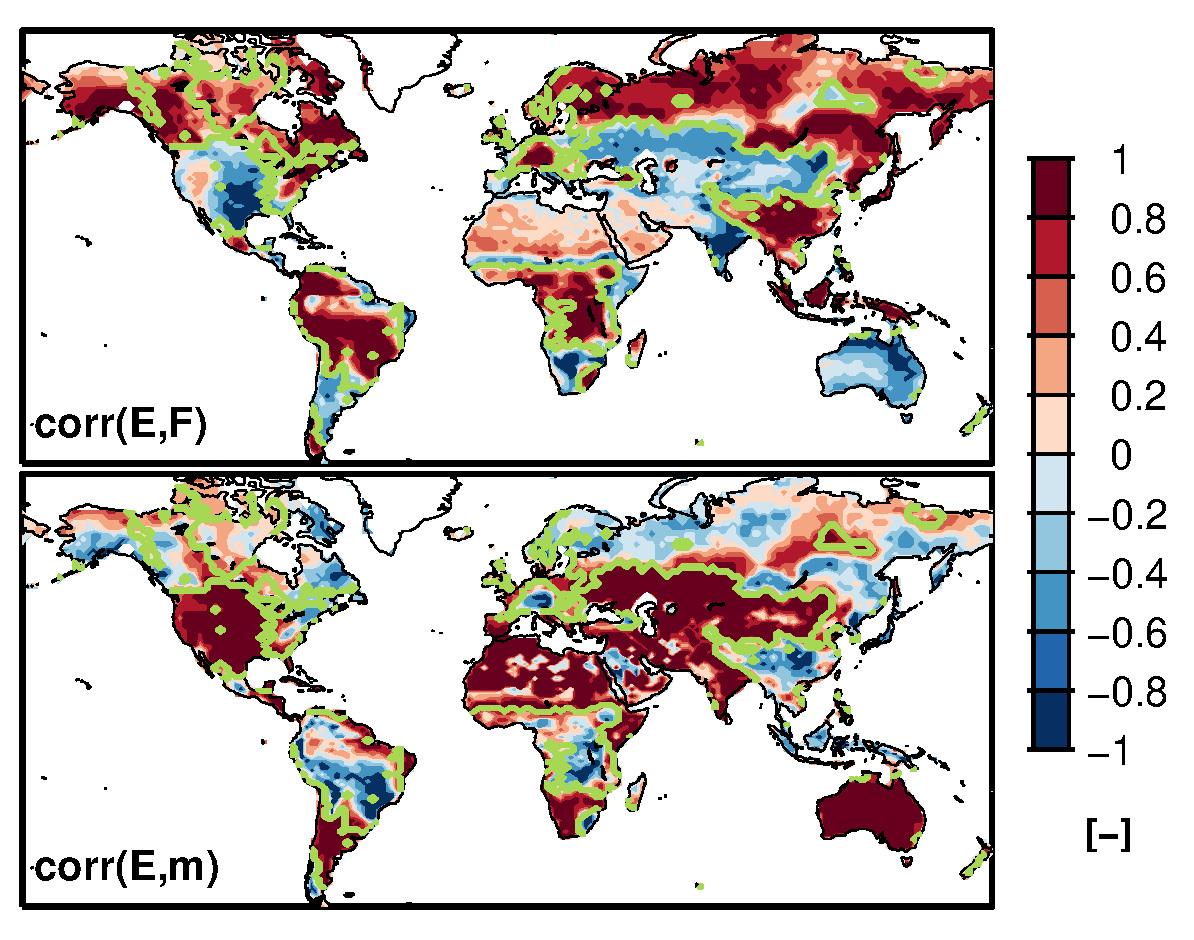
\includegraphics[width=0.6\linewidth]{hadgem1_Cor_EF_Cor_Em_OvGM}}; 
\node[color=colone,font=\bf] at (superposed) 
  {$\mbar\;=\;$ global mean value};
\node[color=p-1,scale=1.5] at (p-1) {\textbullet};
\node[color=p-1,scale=1.5] at (p-11) {\textbullet}; }

% wet point pt
\uncover<4->{%
%
\node[color=p-1,scale=1.5] at (p-2) {\textbullet};
\node[color=p-1,scale=1.5] at (p-22) {\textbullet};  }

\end{tikzpicture}

\end{frame}

\begin{frame}
\frametitle{Correlations {\normalsize involving Evapotranspiration\; (2/2)}}

\begin{columns}

\begin{column}{0.45\linewidth}

\vspace*{-2em}

\begin{itemize}

\item<1-> Decompose radiation forcing anomalies into \\ 
\textcolorbf{colone}{non-precipitating} and \\ 
\textcolorbf{colone}{precipitating} components:

\begin{equation}
  F' \;=\; F_0' \;-\; L\alpha\,  P'
\end{equation}

where $\innerp{F_0'}{P'}\equiv0$, \\ 
$\alpha>0$ (unitless)

%\item<3-> \textcolorbf{colone}{superpose the line where \\ 
%$\mbar$ is equal to the \\ 
%global mean value}

\boxitem[0.82][<3->]{%
%
\textcolorbf{coltwo}{Over dry soils: $F'{>}0$ \\ 
\hspace*{1ex} $\iff$ moisture deficit} \\[0.5em]
%
\textcolorbf{coltwo}{Over wet soils: $m'{>}0$ \\
\hspace*{1ex} $\iff$ energy deficit} }

\end{itemize}

\end{column}

\hfill

\begin{column}{0.52\linewidth}

\vspace*{-0.5em}
\tikzfig{hadgem1_Cor_EF_Cor_Em_Cor_EF0_OvGM}{width=\linewidth}

\end{column}

\end{columns}

\begin{tikzpicture}[overlay]

\coordinate (data) at ($(hadgem1_Cor_EF_Cor_Em_Cor_EF0_OvGM.south)+(-0.4,-0.25)$);

\node[color=colone,font=\bf] at (data) {[\hadgem data]};

\tikzCoverFig[<1>]{hadgem1_Cor_EF_Cor_Em_Cor_EF0_OvGM}{%
  (0,0) rectangle (0.83,0.34)
}

\definecolor{p-1}{RGB}{255,255,51}  % yellow
\coordinate (p-1) at ($(hadgem1_Cor_EF_Cor_Em_Cor_EF0_OvGM.west)+(1.35,2.7)$);
\coordinate (p-11) at ($(hadgem1_Cor_EF_Cor_Em_Cor_EF0_OvGM.west)+(1.35,0.3)$);
\coordinate (p-111) at ($(hadgem1_Cor_EF_Cor_Em_Cor_EF0_OvGM.west)+(1.35,-2.15)$);
\uncover<2>{%
%
\node[color=p-1,scale=1.5] at (p-1) {\textbullet};
\node[color=p-1,scale=1.5] at (p-11) {\textbullet};
\node[color=p-1,scale=1.5] at (p-111) {\textbullet}; }

\end{tikzpicture}

\end{frame}

% -------------------------------------------------------------------------------

%
% Section 3: Toy model
%
%   # of slides: 7 (new 10-15!)
%
% -------------------------------------------------------------------------------
\section{Developing the Toy Model}
\label{sec:toy_model}

\begin{frame}
\frametitle{Toy model preliminaries}

\begin{itemize}

\boxitem{%
%
\textcolorbf{colone}{Goal:} 
%
\parbox{0.8\linewidth}{\centering\textcolorbf{colone}{%
Form an expression for $\Var(T)$.} } }

%\boxitem{% Does not work: leading item is misplaced
\item
%
\quad\textcolorbf{colone}{Tools:} \quad
%
\parbox{0.8\linewidth}{
%
\begin{itemize}
\itemDiamond Surface energy budget,
\itemDiamond Soil moisture budget,  
\itemDiamond Parameterization of land surface fluxes.
\end{itemize}
%
}

\boxitem{%
%
Focus on inter-annual variability: \\[1ex]
--- Use monthly-averaged variables, \\
--- Decompose each variable around monthly climatology:
\begin{equation}
%
  X_{i,j}' \;\equiv\; X_{i,j} \;-\; \Xbar_j
%
\end{equation}
%
\quad where $i\,$: year index, $j\,$: month index.
}

\end{itemize}

\end{frame}

\begin{frame}
\frametitle{Toy model preliminary results}

% define style for equation 
\tikzset{crossout/.style={% 
  draw,ultra thick,cross out,minimum width=4ex,minimum height=4ex,color=coltwo}}

\vspace*{-2em}
Surface energy and soil moisture anomaly budgets:
\vspace*{1.5em}

\setlength{\fboxsep}{6pt}
\Ovalbox{\parbox{0.94\linewidth}{%
%
\begin{subequations}
\vspace*{-1em}
\begin{align}
%
%
  \tikzeqMark{dUdt}{\displaystyle \derv{}{t}\,\big(\pt C\subt{eff}\pt T' \pt\big)} 
  \;\;&=\;\;
%  
  F' \;-\; L\pt E' \;-\; H_s' \;-\; \Fluu \;-\; G' \\
%
  \tikzeqMark{dmdt}{\displaystyle \derv{m'}{t}} \;\;&=\;\;
% 
  P' \;-\; E' \;-\; R' \;-\; I' 
\end{align}
\vspace*{-1em}
\end{subequations} }}

\begin{center}
\vspace*{4em} 
\tikzitemMark
\end{center}

\begin{tikzpicture}[overlay]

% 1) define P, R and I
\tikzitem[<1>]{\parbox{0.8\textwidth}{\centering%
%
$T\;$: 2-meter temperature \enskip, \\[1em]
$C\subt{eff}\;$: effective heat capacity of land surface \enskip, \\[1.5em]
$P\;$: Precipitation \enskip,\enskip 
$R\;$: Surface Runoff \enskip,\enskip
$I\;$: Infiltration \enskip. }}

% 2) choose the surface layer 10\cm moisture content: 
% best correlated, similar autocorrelation properties.
\tikzitem[<2>]{\parbox[t]{0.8\textwidth}{\centering
%
\textcolorbf{colone}{Assume that} $m\,$ is the moisture content \\[0.5em]
in the \textcolorbf{colone}{top 10\cm of soil} }}
%
%\quad\parbox{0.5\textwidth}{
%\begin{itemize}
%\itemDiamond best correlated with $E$, 
%\itemDiamond GCM output.
%%\itemDiamond similar autocorrelation than $T'$.
%\end{itemize} } } }

% 3) One can show that storage terms are small 
\tikzitem[<3>]{%
%
Scale analysis reveals that both
\textcolorbf{colone}{storage terms are negligible}.}

\uncover<3->{%
%
\node[crossout] at (dUdt) {};
\node[crossout] at (dmdt) {}; }

% 4) Define non-GCM outputs G' and I' !
\tikzitem[<4>]{%
%
\textcolorbf{colone}{Define} \enskip $G'\equiv F' - LE' - H_s' - \Fluu$ %
%
\enskip and \enskip % 
%
$I' \equiv P' - E' - R'$ }

% (maybe) inconsistency of E' and top layer

\end{tikzpicture}

\end{frame}

\begin{frame}
\frametitle{Toy model assumptions}

\vspace*{-3em}
\begin{center}

% input from figures/diagrams
\ifdraft{}{%
%
\resizebox{\linewidth}{!}{\begin{tikzpicture}
%
% Land-surface system for the 'toy model assumption slide'
%
% requires the following tikz libraries:
%   arrows, calc, decorations.pathmorphing, shapes
%
%  and package \usepackage[svgnames]{xcolor}
% -----------------------------------------------------------------------------

%% Color and style definitions

% color definition 
\colorlet{sfc}{green!40!black}
\colorlet{landatm}{gray!20!white}
\colorlet{F}{Crimson}
\colorlet{resp}{MidnightBlue}

% box and boundary styles
\tikzset{
  sfc/.style={thick,
              color=sfc},
  sys/.style={fill=landatm,
             rounded corners=2pt},
}

% arrow styles
\tikzset{
  axis/.style={thick,|<->|,font={\sf},left},
  axis2/.style={thick,<->|,font={\sf},left},
  forc/.style={very thick,->,},
  flux/.style={very thick,->,
              scale=1,midway,left,
              decorate,decoration={coil,amplitude=4pt,segment length=7pt}},
  rad/.style={very thick,->,
               decorate,decoration={snake,segment length=17pt}},
  }

% node styles
\tikzset{
    words/.style={font=\sf,scale=0.8},
    symbol/.style={scale=1.1,midway,left,yshift=2ex,color=black},
    param/.style={scale=1.1,above,right,color=black},
}

% -------------------------------------------------------------------------------

%% Coordinates 

% Origin and total width
\coordinate (O) at (0,0);
\pgfmathsetlengthmacro{\W}{10cm}

% Coordinates of sfc, box and axis
\pgfmathsetlengthmacro{\soilH}{0.3cm}
\pgfmathsetlengthmacro{\atmH}{0.7cm}
\coordinate (sfc) at (O);
\coordinate (sfc') at ($(O)+(\W,0)$);
\coordinate (box) at ($(O)-(0,\soilH)$);
\coordinate (box') at ($(O)+(\W,\atmH)$);
\coordinate (axis) at ($(-0.6,-\soilH)$);
\coordinate (axis') at ($(-0.6,0)$);
\coordinate (axis'') at ($(-0.6,\atmH)$);


% Forcing functions coordinates
\coordinate (P) at (2,2);
\coordinate (P') at ($(2,\atmH)+(0,0.05)$);
\coordinate (F0) at (3,2);
\coordinate (F0') at ($(3,\atmH)+(0,0.05)$);

% Fluxes coordinates
\coordinate (E) at ($(4,\atmH-0.65cm)$);
\coordinate (E') at (4.2,1.51);
\coordinate (Hs) at ($(6,\atmH-0.65cm)$);
\coordinate (Hs') at (6.2,1.51);

% Longwave up and heat diffusion
\coordinate (Flu) at ($(8,\atmH-0.65cm)$);
\coordinate (Flu') at (8,1.51);
\coordinate (G) at ($(5,\atmH-0.5cm)$);
\coordinate (G') at (5,-0.7);

% Runoff and infiltration
\coordinate (I) at ($(7,\atmH-0.5cm)$);
\coordinate (I') at (7,-0.7);
\coordinate (R) at (9.5,0.1);
\coordinate (R') at (10.5,0.1);

% -----------------------------------------------------------------------------
	
% -) Drawing the axis
\draw[axis] (axis) -- (axis') node[xshift=-0.6ex,yshift=-7pt] {10 cm};
\draw[axis2] (axis') -- (axis'') node[xshift=-0.6ex] {2 m};

% -) Drawing the atmosphere box
\filldraw[sys] (box) rectangle (box');

% -) Drawing the surface axis and hashes
\draw[sfc] (sfc) -- (sfc');
\foreach \x in {1,...,10}
      \draw[sfc] ($(\x,-5pt)-(0.3,0)$) -- ($(\x,0pt)-(0.6,0)$); 
\node[scale=1.1] at ($(O)+(0.07*\W,7pt)$) {$T'\pt,\pt m'$};

% -) Forcing functions
\draw[forc,color=F] (F0) -- (F0') node[symbol] {$P'$};
\draw[forc,color=F] (P) -- (P') node[symbol] {$F'$};

% -) Fluxes 
\draw[flux,color=resp] (E) -- (E') node[param] {$E'$};
\draw[flux,color=resp] (Hs) -- (Hs') node[param] {$H_s'$};

% -) Longwave up and heat diffusion
\draw[rad,color=resp] (Flu) -- (Flu') node[param] {$\Fluu$};
\draw[rad,color=resp] (G) -- (G') node[param] {$G'$};

% -) Runoff and infiltration
\draw[forc,color=resp] (I) -- (I') node[param] {$I'$};
\draw[forc,color=resp] (R) -- (R') node[param] {$R'$};

\end{tikzpicture}
} }

%\vspace*{1em}

\end{center}

\hfill\parbox{0.9\textwidth}{%
%
\begin{itemize}
%
\item \textcolorbf{colone}{1.\;}\qquad\parbox{0.75\textwidth}{%
%
$F'$ and $P'$ are \textcolorbf{colone}{external forcings}, \\[0.5em] 
independent of $\,E',H_s',\Fluu,G',I',R'\,$. } \\[1.5em]
%
\item \textcolorbf{colone}{2.\:}\qquad\parbox{0.75\textwidth}{%
%
Parameterize $\,E',H_s',\Fluu,G',I',R'\,$ as \\[0.5em]
%\emph{instantaneous} (on monthly time scales) \\[0.5em]
functions of $\,T',m',F',P'\,$ \textcolorbf{colone}{only}.  }
%
\end{itemize} }


%\begin{tikzpicture}[overlay]
%
%\tikzitem[<2>]{\textcolorbf{colone}{1.\:}\qquad\parbox{0.65\textwidth}{%
%%
%Parameterize $\,E',H_s',\Fluu,G',I',R'\,$ as \\[0.5em]
%%\emph{instantaneous} (on monthly time scales) \\[0.5em]
%functions of $\,T',m',F',P'\,$ only. } }
%
%\tikzitem[<3>]{\textcolorbf{colone}{2.\;}\qquad\parbox{0.65\textwidth}{%
%%
%$F'$ and $P'$ are \emph{external forcings}, \\[0.5em] 
%independent of $\,E',H_s',\Fluu,G',I',R'\,$. } }
%
%%% - assumption slide (list 4 assumptions as in thesis section 3.3)
%%% 1 'imply'  item ? T' m' = ....
%
%%% maybe ...
%%Land-surface processes' anomalies are independent of soil moisture content
%%below the surface soil layer (top 10\cm from land surface).
%
%\end{tikzpicture}

\end{frame}

\begin{frame}
\frametitle{Toy model method}

\textcolorbf{colone}{Ex:\enskip} Consider $G'$ (ground heat flux):
\vspace*{0.5em}

\begin{itemize}

\boxitem[0.933][<2->]{%
%
\textcolorbf{colone}{Step 1:} \enskip
%
Regress $G'$ onto 4 possible predictors:
%
\begin{equation}
%
G' = G_0' + a Y'
\quad \text{where} \quad Y'= \big\{ \pt T',\,m',\,F'\,,P' \pt \big\}
%
\end{equation}
%
\hspace*{1em} \textcolorbf{colone}{Best predictor} has 
$\min \big[\pt \innerp{G_0'}{G_0'} \pt\big]$ \\[0.7em]
%
\uncover<3->{%
\hspace*{2em} \textcolorbf{coltwo}{\raisebox{0.3ex}{\danger}}\enskip
If \emph{necessary} repeat \textcolorbf{colone}{step 1.} with $G_0'$ }
} 

\vspace*{-0.7em}

\boxitem[0.933][<4->]{%
%
\textcolorbf{colone}{Step 2:} 
\enskip \textcolorbf{coltwo}{\raisebox{0.3ex}{\danger}}\enskip 
If $T'$ is a \emph{candidate} \\[0.5em]
%
\hspace*{0.5em} Substitute $G' = a T'$ into surface energy anomaly budget:
%
\begin{equation}
%
\hat{\!T\,}' = a\inv\, \big[ F' - LE' - H_s' - \Fluu \big]
%
\end{equation}
%
\hspace*{1em} \textcolorbf{colone}{Evaluate performance} with 
$\rms\big[\pt \hat{\!T\,}' - T'\subt{dataset} \pt\big]$ }

%\item<5-> 1 physically consistent algorithm for all datasets

\end{itemize}

\end{frame}

\begin{frame}
\frametitle{Toy model parameterizations}

\vspace*{-2cm}
\begin{center}

% input from figures/diagrams
\ifdraft{}{%
%
\resizebox{\linewidth}{!}{\begin{tikzpicture}
%
% Land-surface system for the 'toy model parameterization slide'
%
% ** includes the '\uncover' commands **
%
% requires the following tikz libraries:
%   arrows, calc, decorations.pathmorphing, shapes
%
%  and package \usepackage[svgnames]{xcolor}
% -----------------------------------------------------------------------------

%% Color and style definitions

% color definition 
\colorlet{sfc}{green!40!black}
\colorlet{landatm}{gray!20!white}
\colorlet{F}{Crimson}
\colorlet{resp}{MidnightBlue}

% box and boundary styles
\tikzset{
  sfc/.style={thick,
              color=sfc},
  sys/.style={fill=landatm,
             rounded corners=2pt},
}

% arrow styles
\tikzset{
  axis/.style={thick,|<->|,font={\sf},left},
  axis2/.style={thick,<->|,font={\sf},left},
  forc/.style={very thick,->,},
  flux/.style={very thick,->,
              scale=1,midway,left,
              decorate,decoration={coil,amplitude=4pt,segment length=7pt}},
  rad/.style={very thick,->,
               decorate,decoration={snake,segment length=17pt}},
  }

% node styles
\tikzset{
    words/.style={font=\sf,scale=0.8},
    symbol/.style={scale=1.1,midway,left,yshift=1ex,color=black},
    paramA/.style={scale=1.1,above,yshift=0ex,color=black},
    paramB/.style={scale=1.1,below,right,yshift=-0ex,color=black},
    paramR/.style={scale=1.1,above,xshift=2ex,yshift=1ex,color=black},
}

% -------------------------------------------------------------------------------

%% Coordinates 

% Origin and total width
\coordinate (O) at (0,0);
\pgfmathsetlengthmacro{\W}{10cm}

% Coordinates of sfc, box and axis
\pgfmathsetlengthmacro{\soilH}{0.3cm}
\pgfmathsetlengthmacro{\atmH}{0.7cm}
\coordinate (sfc) at (O);
\coordinate (sfc') at ($(O)+(\W,0)$);
\coordinate (box) at ($(O)-(0,\soilH)$);
\coordinate (box') at ($(O)+(\W,\atmH)$);
\coordinate (axis) at ($(-0.6,-\soilH)$);
\coordinate (axis') at ($(-0.6,0)$);
\coordinate (axis'') at ($(-0.6,\atmH)$);

% Forcing functions coordinates
\coordinate (P) at (2,2);
\coordinate (P') at ($(2,\atmH)+(0,0.05)$);
\coordinate (F0) at (3,2);
\coordinate (F0') at ($(3,\atmH)+(0,0.05)$);

% Fluxes coordinates
\coordinate (E) at ($(4,\atmH-0.65cm)$);
\coordinate (E') at (4.2,1.51);
\coordinate (Hs) at ($(6,\atmH-0.65cm)$);
\coordinate (Hs') at (6.2,1.51);

% Longwave up and heat diffusion
\coordinate (Flu) at ($(8,\atmH-0.65cm)$);
\coordinate (Flu') at (8,1.51);
\coordinate (G) at ($(5,\atmH-0.5cm)$);
\coordinate (G') at (5,-0.7);

% Runoff and infiltration
\coordinate (I) at ($(7,\atmH-0.5cm)$);
\coordinate (I') at (7,-0.7);
\coordinate (R) at (9.5,0.1);
\coordinate (R') at (10.5,0.1);

% -----------------------------------------------------------------------------
	
% -) Drawing the axis
\draw[axis] (axis) -- (axis') node[xshift=-0.6ex,yshift=-7pt] {10 cm};
\draw[axis2] (axis') -- (axis'') node[xshift=-0.6ex] {2 m};

% -) Drawing the atmosphere box
\filldraw[sys] (box) rectangle (box');

% -) Drawing the surface axis and hashes
\draw[sfc] (sfc) -- (sfc');
\foreach \x in {1,...,10}
      \draw[sfc] ($(\x,-5pt)-(0.3,0)$) -- ($(\x,0pt)-(0.6,0)$); 
\node[scale=1.1] at ($(O)+(0.07*\W,7pt)$) {$T'\pt,\pt m'$};

% -) Forcing functions
\draw[forc,color=F] (F0) -- (F0') node[symbol] {$P'$};
\draw[forc,color=F] (P) -- (P') node[symbol] {$F'$};

% -) Draw all land-surface processes' arrows
\draw[rad,color=resp] (Flu) -- (Flu');
\draw[rad,color=resp] (G) -- (G');
\draw[flux,color=resp] (E) -- (E');
\draw[flux,color=resp] (Hs) -- (Hs');
\draw[forc,color=resp] (I) -- (I');
\draw[forc,color=resp] (R) -- (R');

% -------------------------------------------------------------------------------

% 1) Longwave up 
\uncover<2->{%
%
\node[paramB] at (Flu') {$\Fluu \,\sim\, T'$}; }

% 2) heat diffusion
\uncover<2->{%
%
\node[paramB] at (G') {$G' \,\sim\, T'$}; }

% 3) Runoff 
\uncover<2->{%
%
\node[paramR] at (R') {$R' \,\sim\, P'$}; }

% 4) Infiltration
\uncover<3->{%
%
\node[paramB] at (I') {$I' \,\sim\, (m',P')$}; }

% 5) Evapotranspiration
\uncover<4->{%
%
\node[paramA,xshift=1ex] at (E') {$E' \,\sim\, (m',F')$}; }

% 6) Sensible heat flux
\uncover<5->{%
%
\node[paramA,xshift=3.5ex,yshift=1ex] at (Hs') {$H_s' \,\sim\, (T',-{m'})$}; }


\end{tikzpicture}
} }

\vspace*{3em}
\tikzitemMark

%\vfill\hfill\parbox{0.8\textwidth}{%
%%
%$\gamma$, $\lambda$, all $\nu$'s and $\beta$ 
%\textcolorbf{colone}{are positive definite} }

\end{center}

\begin{tikzpicture}[overlay]

% for the Flu', G', I'
\tikzitem[<2>]{%
%
3 out of 6 processes were \emph{easy} to parameterize}

% for the I' item
\tikzitem[<3>]{\parbox{0.6\textwidth}{\centering%
%
2 predictors for inflitration $m'$ and $P'$ }}

% for the E' item
\tikzitem[<4>]{\parbox{0.87\textwidth}{\centering%
%
Special algorithm for $E'$ to model both $E$ regimes: \\[1.5em]%
\textcolorbf{colone}{If} $\innerp{E'}{m'}>0$\,:\enskip 
2 predictors $m'\,$ and $F'\,$ (moisture-limited) \\[1em] 
\hspace*{-2.5em} \textcolorbf{colone}{Otherwise:} 
\hspace*{0.8em} 1 predictor $F'$ only (energy-limited)} }

% for the H_s' term
\tikzitem[<5>]{\parbox{0.8\textwidth}{\centering%
%
\textcolorbf{coltwo}{Surprising result:} 
$H_s'$ is best predicted by $m'\,$!\\[1.5em]
Use 2 predictors $T'$ and $m'$ }}

\end{tikzpicture}

\end{frame}

\begin{frame}
\frametitle{Toy model {\large expressions / coefficients}}

% define style for equation 
\tikzset{term/.style={%
  rounded corners=2pt, minimum height=4ex, minimum width=4ex, 
  fill=MidnightBlue!40}}

\vspace*{-2em}
After some algebra:
\vspace*{1em}

\setlength{\fboxsep}{10pt}
\Ovalbox{\parbox{0.94\linewidth}{%
%
\begin{subequations}
\begin{align}
%
 \Ttm \;&=\; 
%
\tikzeqMark{gamma}{\displaystyle \frac{1}{\;\gamma\;} }
%
 \, \Big[ \,\big( \pt 1
%
\tikzeqMark{lambda-1}{\displaystyle -\,\lambda} 
%  
 \pt \big)\, F_0'
%
 \;-\; L\alpha \big( \pt 1
%
\tikzeqMark{lambda-2}{\displaystyle -\,\lambda}
% 
 \pt \big)\, P' \;-\; L\, 
% 
\tikzeqMark{effects-m}{\displaystyle \big( \pt \nuE - \nuHs \pt \big)\, m'}
%
 \, \Big] \\
%
 \tikzeqMark{mtm}{\displaystyle \mtm}  \;&=\; 
%
 \tikzeqMark{nus}{\displaystyle \frac{1}{\;\nuI+\nuE\;}} 
% 
 \, \Big[ \, \big( \pt 1 
%
\tikzeqMark{lambda-3}{\displaystyle +\,\alpha \lambda} 
%
\tikzeqMark{beta}{\displaystyle -\,\beta}
% 
 \pt \big)\, P' \;-\; 
%
 \tikzeqMark{lambda-4}{\displaystyle \big( \pt \tfrac{\lambda}{L} \pt \big)}  
%
 \, F_0' \, \Big] 
%
\end{align}
\end{subequations} } }

\begin{center}

\vspace*{3em}
\tikzitemMark

\end{center}

\begin{tikzpicture}[overlay]

\tikzitem[<1>]{\textcolorbf{colone}{Recall} \quad \parbox{0.55\textwidth}{%
%
$F'=F_0' - L\alpha P'$ \\[1ex]
$L$ : specific latent heat of vaporization} }

% gamma
\tikzitem[<2>]{\textcolorbf{colone}{Surface temperature resistance}
\enskip ($\Wm[-2]\K[-1]$)}
%
\uncover<2>{%
%
\node[term] at (gamma) {$\displaystyle \frac{1}{\;\gamma\;}$}; }

% lambda
\tikzitem[<3>]{\textcolorbf{colone}{Evapotranspiration efficiency} 
\enskip (unitless)}
%
\uncover<3>{%
%
\node[term] at (lambda-1) {$\displaystyle -\,\lambda$}; 
\node[term] at (lambda-2) {$\displaystyle -\,\lambda$}; 
\node[term] at (lambda-3) {$\displaystyle +\,\alpha\lambda$}; 
\node[term] at (lambda-4) 
  {$\displaystyle \big(\pt \tfrac{\lambda}{L} \pt\big)$}; }

% beta 
\tikzitem[<4>]{\textcolorbf{colone}{Fraction of $P'$ loss to $I'$ and $R'$} 
\enskip (unitless)}
%
\uncover<4>{%
%
\node[term] at (beta) {$\displaystyle -\,\beta$}; }

% nu E - nu H_s
\tikzitem[<5>]{\parbox{0.7\textwidth}{\centering
\textcolorbf{colone}{Net effect of soil moisture anomalies on $T'$} \\[1em]
All $\nu$'s have units of $\s[-1]$} }
%
\uncover<5>{%
%
\node[term] at (effects-m) 
  {$\displaystyle \big( \pt \nuE - \nuHs \pt \big)\, m'$}; }

% define chi
\tikzitem[<6>]{\parbox{0.82\textwidth}{\centering%
\textcolorbf{colone}{Define}\quad
$\displaystyle \chi \equiv \frac{\nuE-\nuHs}{\nuI+\nuE}$ 
\enskip (unitless) \enskip
\textcolorbf{colone}{the coupling coefficient} \\[1em]
Modulates net effect of $m'$ on $T'$ } }
%
\uncover<6>{%
%
\node[term] at (effects-m) 
  {$\displaystyle \big( \pt \nuE - \nuHs \pt \big)\, m'$};
\node[term] at (mtm) {$\displaystyle \mtm$};
\node[term] at (nus) {$\displaystyle \frac{1}{\;\nuI+\nuE\;}$}; }

%% Combine gamma and beta
%\tikzitem[<6>]{\quad\parbox{0.85\textwidth}{%
%%
%$\gamma\;$: [$\Wm[-2]\K[-1]$] \hspace*{2em}
%%
%\parbox{0.65\textwidth}{%
%%
%from param. $\Fluu \,,\, H_s' \,,\, G'$  onto $T'$ \\[1ex]
%%
%\hspace*{1em} } \\[1.5em]
%%
%$\beta\;$: [unitless] \hspace*{3em}
%%
%\parbox{0.65\textwidth}{%
%%
%from param. $I' \,,\, R'$ onto $P'$ \\[1ex]
%%
%\hspace*{1em} 
%%
%} }
%
%%% Lambda and nu's
%\tikzitem[<7>]{\quad\parbox{0.85\textwidth}{%
%%
%$\lambda\;$: [unitless] \hspace*{3em}
%%
%\parbox{0.65\textwidth}{%
%%
%from param. $E'$ onto $F'$ \\[1ex]
%%
%\hspace*{1em} 
%%
%$\nuE \,,\, \nuHs \,,\, \nuI\;$: [\s[-1]] \hspace*{1em}
%%
%\parbox{0.65\textwidth}{%
%%
%from param. $E' \,,\, (-H_s') \,,\, I'$ onto $m'$ \\[1em]
%%
%\hspace*{1em} 
%\textcolorbf{colone}{rate at which $m'$ induces $E' \,,\, (-H_s') \,,\, I'$} }
%%
%} }


\end{tikzpicture}


\end{frame}

\begin{frame}
\frametitle{Toy model performance}

\begin{center}

% 1) world map
\uncover<1>{%
%
\tikzfig{comp_tm_Var_T_bias}{width=\textwidth} }

\tikzitemMark

\end{center}

\begin{tikzpicture}[overlay]

\coordinate (title) at ($(comp_tm_Var_T_bias.north)+(-0.4,0.4)$);
\coordinate (label1) at ($(comp_tm_Var_T_bias.west)+(2,1)$);
\coordinate (label2) at ($(comp_tm_Var_T_bias.south east)+(-1.5,0.5)$);

% write Var(T) expression over figure
\node[color=colone,font=\bf] at (title) 
  {\small $\displaystyle \VarTtm = 
    \frac{1}{\gamma^2}\, \Big[ 
      \big( 1-\lambda(1-\chi) \big)^2 \Var(F_0) + 
      L^2 \big( \alpha(1-\lambda)+\chi(1+\alpha\lambda-\beta) \big)^2 \Var(P)
     \Big]$ };

\tikzitem[<1>]{%
Plotted as \enskip $\dfrac{\VarTtm}{\Var(T\subt{dataset})}$ }

% 2) histogram of all land points
\uncover<2->{%
%
\node at (comp_tm_Var_T_bias) {%
  \includegraphics[trim=0cm 0.5cm 0cm 0.72cm,clip,width=0.55\textwidth]%
  {hist_comp_tm_Var_T_bias}}; 
\node[font=\bf] at (label1) {Probability};
\node[font=\bf] at (label2) 
  {$\dfrac{\VarTtm}{\Var(T\subt{dataset})}$};
%
}

\tikzitemImply[<2>]{\textcolorbf{coltwo}{%
%
Toy model underestimates dataset outputs by $\sim$ 20\% to 40\%. } }

%% Why underestimation ? 
% - soil moisture, H_s parameterization, neglected processes (memory, feedbacks)

%% bin size ? 0.025.

\end{tikzpicture}

\end{frame}

% -------------------------------------------------------------------------------

%
% Section 4: Interpretation
%
%   # of slides: 6 (new 10-20!) 
%
% -------------------------------------------------------------------------------
\section{Toy Model Interpretation}
\label{sec:interpret}

\begin{frame}
\frametitle{Interpreting the Toy Model}

Toy model expresses \enskip 
$\Var(T) = \mcal{F}\big(\Var(F_0),\Var(P),\,\text{\tmcoeffs}\big)$

\vspace*{1em}

\begin{itemize}

% Q for coefficients -- mean state
\boxitem[0.88][<1->]{%
%
\textcolorbf{colone}{Q:} \quad
%
\parbox{0.68\linewidth}{\centering
Do the \tmcoeffs \\ show dependence \\ on mean-state variables ? }
%
\uncover<2->{\quad \textcolorbf{colone}{Not today!} } }

% Q for relative contribution of forcing to variance
\boxitem[0.88][<1->]{%
%
\textcolorbf{colone}{Q:} \quad
%
\parbox{0.68\linewidth}{\centering
What are the relative contributions \\ 
of $\Var(F_0)$ and $\Var(P)$ to $\Var(T)$ ?}
%
\uncover<2->{\quad \textcolorbf{colone}{Not today!} } }

% Q for role of land-surface on Var(T)
\boxitem[0.88][<2->]{%
%
\textcolorbf{colone}{Q:} \quad
%
\parbox{0.8\linewidth}{\centering\textcolorbf{colone}{%
What is the role of soil moisture \\ 
(mean-state and anomalies) on $\Var(T)$ ?} } }

\end{itemize}

\end{frame}

\begin{frame} 
\frametitle{{\large Role of the land surface on surface temperature variability}}

\vspace*{-1.5em}

\begin{itemize}

\item<1-> Start from the toy model expression for $\Var(T)$: 
%
\begin{equation*}
%
\hspace*{-1em}
%
  \VarTtm = \frac{1}{\gamma^2}\, \Big[ 
  \big( 1-\textcolor{colone}{\lambda}(1-\textcolor{colone}{\chi}) \big)^2 \Var(F_0) + 
  L^2 \big( \alpha(1-\textcolor{colone}{\lambda})+
   \textcolor{colone}{\chi}(1+\alpha\lambda-\beta) \big)^2 \Var(P)
  \Big] 
%
\end{equation*}

\boxitem[0.88][<2->]{%
%
\textcolorbf{colone}{Set} \qquad
%
\parbox{0.75\linewidth}{
\textcolor{colone}{$\chi$} 
  {\small (effects of soil moisture anomalies on $\Var(T)$)} \\
\textcolor{colone}{$\lambda$} 
  {\small (evapotranspiration efficiency)} }
%
\textcolor{colone}{$\displaystyle = 0$} \\[1.5em]
%
\textcolorbf{colone}{To get:} \qquad
$\displaystyle \VarTtm = \gamma\invv \big[ \Var(F_0) + L^2\alpha^2\Var(P) \big]$
}

\boxitem[0.88][<3->]{\textcolorbf{colone}{Define} \enskip 
%
$\dfrac{\gamma^2\Var(T)}{\Var(F)}$ \enskip 
\textcolorbf{colone}{the surface temperature response} }

\end{itemize}

\end{frame}

\begin{frame}
\frametitle{Two regimes {\large of surface temperature variability}}

\begin{center}

\uncover<1>{%
%
\tikzfig{comp_scale_gammaT}{width=\textwidth} }

\tikzitemMark

\end{center}

\begin{tikzpicture}[overlay]

\coordinate (title) at ($(comp_scale_gammaT.north)+(-0.4,0.4)$);
\node[color=colone,font=\bf] at (title) 
  {Surface temperature response $\gamma^2\Var(T)/\Var(F)$};

% - Surface temperature variability
%   land-surface amplified / damped regimes !!!
\tikzitem[<1>]{\parbox{0.8\linewidth}{\centering%
%
The land surface is able to \\
\textcolorbf{colone}{amplify} and \textcolorbf{colone}{damp} \\
surface temperature variability} }

% show comp_scale_gammaT (with and without global mean soil moisture)
\uncover<2->{%
%
\node at (comp_scale_gammaT) 
  {\includegraphics[width=\textwidth]{comp_scale_gammaT_OvGM}} ; }

\tikzitem[<2>]{\parbox{0.8\linewidth}{\centering%
%
Superpose with global mean soil moisture contour: \\[1ex]
\textcolorbf{coltwo}{Dry soils}
(moisture-limited $E$) 
\textcolorbf{coltwo}{amplify $\Var(T)$}, \\
\textcolorbf{coltwo}{Wet soils} 
(energy-limited $E$)
\textcolorbf{coltwo}{damp $\Var(T)$ } } }

\end{tikzpicture}

\end{frame}

\begin{frame}
\frametitle{Interpret: {\large Land-surface amplified / Moisture-limited}}

\vspace*{-1.5em}

\begin{itemize}

\itemDiamond $\lambda\;$: evapotranspiration efficiency 

\itemDiamond $\chi\;$: coupling coefficient (modulates net effect of $m'$ on $T'$)

\end{itemize}

\begin{center}

% input from figures/diagrams
\ifdraft{}{%
%
\resizebox{\linewidth}{!}{\begin{tikzpicture}
%
% Land-surface damped summary diagram. 
%
% ** include 'uncover' tikz commands **
%
% requires the following tikz libraries:
%   arrows, calc, decorations.pathmorphing, shapes
% 
%   and the 'wasysym' package
% -----------------------------------------------------------------------------

%% Styles and colors

% Color definition (requires \usepackage[svgnames]{xcolor})
\colorlet{sfc}{colone}
\colorlet{landatm}{gray!20!white}
\colorlet{F}{black}
\colorlet{proc}{black}
\colorlet{warm}{Crimson}
\colorlet{cold}{MidnightBlue}

% Box and boundary styles
\tikzset{
  sfc/.style={thick,
              color=sfc},
  sys/.style={fill=landatm,
             rounded corners=2pt},
}

% Arrow styles
\tikzset{
  axis/.style={thick,|<->|,font={\scriptsize \sf},left},
  axis2/.style={thick,<->|,font={\scriptsize \sf},left},
  forc/.style={very thick,->,},
  flux/.style={very thick,->,
              scale=0.8,midway,left,
              decorate,decoration={coil,amplitude=4pt,segment length=7pt}},
  rad/.style={very thick,->,
               decorate,decoration={snake,segment length=17pt}},
}

% Node styles
\tikzset{
    symbol/.style={scale=0.8,midway,left,yshift=1ex,color=black},
    param/.style={scale=0.7,color=black},
    coef/.style={scale=0.8,color=black},
    resp/.style={scale=0.8,draw,very thick,ellipse,fill=landatm},
}

% -------------------------------------------------------------------------------

%% Coordinates, lengths

% Origin, box width, gap in-between box
\coordinate (O) at (0,0);
\pgfmathsetlengthmacro{\W}{5cm}
\pgfmathsetlengthmacro{\gap}{0.5cm}

% Length for soil height, atm height, above sfc text
\pgfmathsetlengthmacro{\soilH}{0.3cm}
\pgfmathsetlengthmacro{\atmH}{0.7cm}
\pgfmathsetlengthmacro{\Asfc}{0.3cm}

% left-hand land-atm box
\coordinate (sfc1) at (O);
\coordinate (sfc1') at ($(sfc1)+(\W,0)$);
\coordinate (box1) at ($(sfc1)-(0,\soilH)$);
\coordinate (box1') at ($(sfc1)+(\W,\atmH)$);

% right-hand land-atm box
\coordinate (sfc2) at ($(sfc1')+(\gap,0)$);
\coordinate (sfc2') at ($(sfc2)+(\W,0)$);
\coordinate (box2) at ($(sfc2)-(0,\soilH)$);
\coordinate (box2') at ($(sfc2)+(\W,\atmH)$);

% 'F0' box coordinates
\coordinate (F0) at (1.5,2);
\coordinate (F0') at ($(1.5,\atmH)+(0,0.05)$);
\coordinate (lambda) at ($(1.5,\Asfc)$);
\coordinate (T1) at ($(3.5,\Asfc)$);

% 'P' box coordinate
\coordinate (P) at ($(1.5,2)+(\W,0)+(\gap,0)$);
\coordinate (P') at ($(1.5,\atmH)+(0,0.05)+(\W,0)+(\gap,0)$);
\coordinate (I) at ($(1.5,0)+(\W,0)+(\gap,\atmH-0.5cm)$);
\coordinate (I') at ($(1.5,0)+(\W,0)+(\gap,-0.7)$);
\coordinate (R) at ($(1,0)+(\W,0)+(\gap,0.25)$);
\coordinate (R') at ($(-0.2,0)+(\W,0)+(\gap,0.25)$);
\coordinate (E) at ($(2.1,0)+(\W+\gap,0.35)+(0,\atmH-0.5cm)$);
\coordinate (E') at ($(2.3,0)+(\W+\gap,0)+(0,1.51)$);
\coordinate (m2) at ($(1.5,0)+(\W,0)+(\gap,\Asfc)$);
\coordinate (T2) at  ($(3.5,0)+(\W,0)+(\gap,\Asfc)$);
\coordinate (chi) at  ($(2.8,0)+(\W,0.7)+(\gap,\Asfc)$);
%\coordinate (Hs) at ($(2.4,0)+(\W+\gap,0)+(0,\atmH-0.65cm)$);
%\coordinate (Hs') at ($(2.6,0)+(\W+\gap,0)+(0,1.51)$);
%\coordinate (dT1) at ($(3.2,0)+(\W,0.1)+(\gap,\Asfc)$);

% -----------------------------------------------------------------------------

% 1a) drawing the 'F0' box , F0 positive , lambda small
\uncover<1->{%
%
\filldraw[sys] (box1) rectangle (box1');
\draw[sfc] (sfc1) -- (sfc1');
\foreach \x in {1,...,5}
  \draw[sfc] ($(\x,-5pt)-(0.3,0)$) -- ($(\x,0pt)-(0.6,0)$); 
%
\draw[forc,color=warm] (F0) -- (F0') node[symbol] {$F_0'>0$};
%
\node[color=cold,coef] at (lambda) {$\lambda\approx0$};
%
}

% 1b) T response
\uncover<1->{%
%
\node[color=warm,resp] at (T1) {$T'>0$};
%
}

% -------------------------------------------------------------------------------

% 3) drawing the 'P' box , P positive , 
%    lambda=0, m response , infiltration , runoff
\uncover<2->{%
%
\filldraw[sys] (box2) rectangle (box2');
\draw[sfc] (sfc2) -- (sfc2');
\foreach \x in {1,...,5}
  \draw[sfc] ($(\x,-5pt)+(0.1,0)+(\W,0)$) -- ($(\x,0pt)-(0.2,0)+(\W,0)$); 
%
\draw[color=cold,forc] (P) -- (P') node[symbol] {$\alpha P'>0$};
%
%\draw[forc,color=proc] (I) -- (I') node[param,below] {$I'>0$};
%
%\draw[forc,color=proc] (R) -- (R') node[param,above,xshift=2.5em] {$R'>0$};
%
\node[resp] at (m2) {$m'>0$};   % rust overlay others paths/nodes
%
\node[scale=0.7,xshift=1.5em] at (chi) {$\lambda\approx0$};
}

% 4) evaporation and sensible heat , chi positive , T response
\uncover<3->{%
% 
\draw[flux,color=cold] (E) -- (E') 
  node[param,above,xshift=1em] {$(E'{+}H_s')>0$};
% 
\node[scale=0.7,xshift=4.5em] at (chi) {$,\;\chi>0$};
% 
\node[color=cold,resp] at (T2) {$T'<0$};
%
}

\end{tikzpicture}
} }

\vspace*{1.5em}
\tikzitemMark

\end{center}

\begin{tikzpicture}[overlay]

\tikzitem[<1>]{%
%
Non-precipitating $F'$ are unattenuated by land surface}

\tikzitem[<2>]{%
%
Radiative effects of $P'$ on $E'$ are negligible}

\tikzitem[<3>]{\hfill\parbox{0.9\linewidth}{\centering%
%
Soil moisture input generates latent cooling (via $E$\,) \\[1em]
%
\textcolorbf{coltwo}{%
Radiative effects of $P'$ on $T'$ are amplified by land surface} \\[1em]
%
\textcolorbf{coltwo}{%
Soil moisture anom. amplify $T'$} 
} }

% more ...

\end{tikzpicture}

\end{frame}

\begin{frame}
\frametitle{Interpret: {\large Land-surface damped / Energy-limited}}

\vspace*{-1.5em}

\begin{itemize}

\itemDiamond $\lambda\;$: evapotranspiration efficiency 

\itemDiamond $\chi\;$: coupling coefficient (modulates net effect of $m'$ on $T'$)

\end{itemize}

\begin{center}

%% input from figures/diagrams
\ifdraft{}{%
%
\resizebox{\linewidth}{!}{\input{figures/diagrams/tm_interp_wet}} }

\vspace*{1.5em}
\tikzitemMark

\end{center}

\begin{tikzpicture}[overlay]

\tikzitem[<1>]{\hfill\parbox{0.9\linewidth}{\centering%%
%
$E$\, responds to radiation, 
opposing $F_0'$ and $\alpha P'$ \\[1em]
%
\textcolorbf{coltwo}{%
Radiative effects of $P'$ on $T'$ are damped by land surface} } }

\tikzitem[<2>]{\hfill\parbox{0.9\linewidth}{\centering%
%
Soil moisture anomaly modifies sensible heat flux \\[1em]
%
Further damping $\alpha P'$ } }

% more ...

\end{tikzpicture}

\end{frame}

\begin{frame}
\frametitle{\large Surface temperature variability is regime dependent}

%\vspace*{-2em}

%% input from figures/diagrams
\ifdraft{}{%
%
\resizebox{\linewidth}{!}{\begin{tikzpicture}
%
% Tree diagram summarizing the 'recipe' for surface temperature variability
%
% requires the following tikz libraries:
%   arrows, calc, decorations.pathmorphing, shapes
%
% -----------------------------------------------------------------------------

%% style definitions

\tikzset{%
%
  root/.style={rectangle,draw=black,very thick,rounded corners=2pt,
               align=center,font={\bf \large},fill=colone!60},
  level 1/.style={sibling distance=45mm},
  edge from parent/.style={->,draw,very thick,shorten >=2pt},
  level 2/.style={rounded corners=6pt,align=center,fill=colone!40,
                   text width=12em,font=\bf},
  level 3/.style={align=center,fill=colfl!50,inner sep=2pt,
                  text width=10em,text height=1em},
  level 3m/.style={align=center,fill=colfl!50,inner sep=2pt,
                   text width=6em,text height=0.8em,font={\small}},
  level 4/.style={rectangle,draw=black,very thick,rounded corners=2pt,
                  inner sep=4pt,text height=0.6em,
                  align=center,fill=colone!60,text width=4em,font={\bf}},
  subarrow/.style={thick,arrows=-square,shorten >=3pt},
  mag-arrow/.style={->,very thick,shorten >=2pt},
%
}

% -------------------------------------------------------------------------------

%% 1. Regimes 

\node[root] {2 regimes:}
  child {node[level 2] (c1) 
    {Land-surface amplified \\[0.5ex]
    $\frac{\gamma^2\Var(T)}{\Var(F)}>1$} }
  child {node[level 2] (c2) 
    {Land-surface damped \\[0.5ex]
    $\frac{\gamma^2\Var(T)}{\Var(F)}<1$} };

% -------------------------------------------------------------------------------

%% is associated with

\begin{scope}[every node/.style={level 3}]

  \coordinate (m0) at ($(c1.west) + (-1.2,0)$);
  \coordinate (m1) at ($(c1.south west) + (-1.2,-0.32)$);

  \uncover<2->{%
  %
  \node[level 4] at (m0) {Metrics:}; 
  %
  \node[level 3m,yshift=-10pt] at (m1) {$\sgn(\mbar-m\subt{crit})$};
  \node[level 3m,below of=m1,yshift=-15pt] (m2) {$\sgn(\corr(E,m))$};
  \node[level 3m,below of=m2,yshift=-5pt] (m3) {$\sgn(\corr(E,F))$};
  \node[level 3m,below of=m3,yshift=-5pt] (m4) {$\sgn(\chi)$};
  %
  \node[below of=c1,xshift=5pt,yshift=-10pt] (c11) 
    { {\bf Dry soils} \\ ($<0$) };
  \node[below of=c11,yshift=-5pt] (c12)
    { {\bf Moisture-limited} \\ ($>0$) };
  \node[below of=c12,yshift=-5pt,fill=colbg] (c13) 
    { {\bf \phantom{dsadsa}} \\ \phantom{($<0$)} };
  \node[below of=c13,yshift=-5pt] (c14) 
    { $m'{>}0$ {\bf \small assoc.} $T'{>}0$ \\ ($>0$) };
  %
  \node[below of=c2,xshift=5pt,yshift=-10pt] (c21) 
    { {\bf Wet soils} \\ ($>0$)};
  \node[below of=c21,yshift=-5pt,fill=colbg] (c22) 
    { {\bf \phantom{dsadsa}} \\ \phantom{($>0$)} };
  \node[below of=c22,yshift=-5pt] (c23)
    { {\bf Energy-limited} \\ ($>0$) };
  \node[below of=c23,yshift=-5pt] (c24) 
    { $m'{>}0$ {\bf \small assoc.} $T'{<}0$ \\ ($<0$) };
  %
  }

\end{scope}

% -------------------------------------------------------------------------------

%%% 2. Magnitudes governed by
%
%\begin{scope}[every node/.style={level 4}]
%
%\uncover<2->{%
%%
%  \node[below of=c14,xshift=5pt] (c111) 
%    {2. $\left|\frac{\gamma^2\Var(T)}{\Var(F)}\right|\propto\chi\Var(P)^\half$};
%  \node[below of=c24,xshift=-10pt] (c222) 
%    {2. $\left|\frac{\gamma^2\Var(T)}{\Var(F)}\right|\propto\lambda$ or $\,\mbar$};
%%
%}
%
%\end{scope}
%
%% -------------------------------------------------------------------------------

%% draw lines 

\uncover<2->{%
%
\foreach \value in {1,2,4}
  \draw[subarrow] (c1.200) |- ($(c1\value.west) + (0.4,0)$);
%
\foreach \value in {1,3,4}
  \draw[subarrow] (c2.200) |- ($ (c2\value.west) + (0.4,0)$);
%
}

%\uncover<2->{%
%%
%\path[mag-arrow] (c1.198) edge [bend right] (c111.168);
%\path[mag-arrow] (c2.342) edge [bend left] (c222.12);
%%
%}

% -------------------------------------------------------------------------------

\end{tikzpicture}
} }
%\resizebox{\linewidth}{!}{\begin{tikzpicture}
%
% Tree diagram summarizing the 'recipe' for surface temperature variability
%
% requires the following tikz libraries:
%   arrows, calc, decorations.pathmorphing, shapes
%
% -----------------------------------------------------------------------------

%% style definitions

\tikzset{%
%
  root/.style={rectangle,draw=black,very thick,rounded corners=2pt,
               align=center,font={\bf \large},fill=colone!60},
  level 1/.style={sibling distance=45mm},
  edge from parent/.style={->,draw,very thick,shorten >=2pt},
  level 2/.style={rounded corners=6pt,align=center,fill=colone!40,
                   text width=12em,font=\bf},
  level 3/.style={align=center,fill=colfl!50,inner sep=2pt,
                  text width=10em,text height=1em},
  level 3m/.style={align=center,fill=colfl!50,inner sep=2pt,
                   text width=6em,text height=0.8em,font={\small}},
  level 4/.style={rectangle,draw=black,very thick,rounded corners=2pt,
                  inner sep=4pt,text height=0.6em,
                  align=center,fill=colone!60,text width=4em,font={\bf}},
  subarrow/.style={thick,arrows=-square,shorten >=3pt},
  mag-arrow/.style={->,very thick,shorten >=2pt},
%
}

% -------------------------------------------------------------------------------

%% 1. Regimes 

\node[root] {2 regimes:}
  child {node[level 2] (c1) 
    {Land-surface amplified \\[0.5ex]
    $\frac{\gamma^2\Var(T)}{\Var(F)}>1$} }
  child {node[level 2] (c2) 
    {Land-surface damped \\[0.5ex]
    $\frac{\gamma^2\Var(T)}{\Var(F)}<1$} };

% -------------------------------------------------------------------------------

%% is associated with

\begin{scope}[every node/.style={level 3}]

  \coordinate (m0) at ($(c1.west) + (-1.2,0)$);
  \coordinate (m1) at ($(c1.south west) + (-1.2,-0.32)$);

  \uncover<2->{%
  %
  \node[level 4] at (m0) {Metrics:}; 
  %
  \node[level 3m,yshift=-10pt] at (m1) {$\sgn(\mbar-m\subt{crit})$};
  \node[level 3m,below of=m1,yshift=-15pt] (m2) {$\sgn(\corr(E,m))$};
  \node[level 3m,below of=m2,yshift=-5pt] (m3) {$\sgn(\corr(E,F))$};
  \node[level 3m,below of=m3,yshift=-5pt] (m4) {$\sgn(\chi)$};
  %
  \node[below of=c1,xshift=5pt,yshift=-10pt] (c11) 
    { {\bf Dry soils} \\ ($<0$) };
  \node[below of=c11,yshift=-5pt] (c12)
    { {\bf Moisture-limited} \\ ($>0$) };
  \node[below of=c12,yshift=-5pt,fill=colbg] (c13) 
    { {\bf \phantom{dsadsa}} \\ \phantom{($<0$)} };
  \node[below of=c13,yshift=-5pt] (c14) 
    { $m'{>}0$ {\bf \small assoc.} $T'{>}0$ \\ ($>0$) };
  %
  \node[below of=c2,xshift=5pt,yshift=-10pt] (c21) 
    { {\bf Wet soils} \\ ($>0$)};
  \node[below of=c21,yshift=-5pt,fill=colbg] (c22) 
    { {\bf \phantom{dsadsa}} \\ \phantom{($>0$)} };
  \node[below of=c22,yshift=-5pt] (c23)
    { {\bf Energy-limited} \\ ($>0$) };
  \node[below of=c23,yshift=-5pt] (c24) 
    { $m'{>}0$ {\bf \small assoc.} $T'{<}0$ \\ ($<0$) };
  %
  }

\end{scope}

% -------------------------------------------------------------------------------

%%% 2. Magnitudes governed by
%
%\begin{scope}[every node/.style={level 4}]
%
%\uncover<2->{%
%%
%  \node[below of=c14,xshift=5pt] (c111) 
%    {2. $\left|\frac{\gamma^2\Var(T)}{\Var(F)}\right|\propto\chi\Var(P)^\half$};
%  \node[below of=c24,xshift=-10pt] (c222) 
%    {2. $\left|\frac{\gamma^2\Var(T)}{\Var(F)}\right|\propto\lambda$ or $\,\mbar$};
%%
%}
%
%\end{scope}
%
%% -------------------------------------------------------------------------------

%% draw lines 

\uncover<2->{%
%
\foreach \value in {1,2,4}
  \draw[subarrow] (c1.200) |- ($(c1\value.west) + (0.4,0)$);
%
\foreach \value in {1,3,4}
  \draw[subarrow] (c2.200) |- ($ (c2\value.west) + (0.4,0)$);
%
}

%\uncover<2->{%
%%
%\path[mag-arrow] (c1.198) edge [bend right] (c111.168);
%\path[mag-arrow] (c2.342) edge [bend left] (c222.12);
%%
%}

% -------------------------------------------------------------------------------

\end{tikzpicture}
}

%% within each regimes ...

\end{frame}

% -------------------------------------------------------------------------------

%
% Section 5: Applications
%
%   # of slides: 3 
%
% -------------------------------------------------------------------------------
\section{Toy Model Applications}
\label{sec:apps}

\begin{frame}
\frametitle{Toy Model Applications}

\begin{itemize}

\boxitem[0.88][<1->]{%
%
\textcolorbf{colone}{\large 1.} \quad
%
\parbox{0.68\linewidth}{\centering
Attributing GCM $\Var(T)$ errors to forcings \\[0.5em]
and/or land-atmosphere interactions. } 
%
\quad \textcolorbf{colone}{Not today!} } 

\boxitem[0.88][<1->]{%
%
\textcolorbf{colone}{\large 2.} \quad
%
\parbox{0.8\linewidth}{\centering
\textcolorbf{colone}{Insight on late \twentyfirst century $\Var(T)$
projections.} }}

\end{itemize}

\end{frame}

\begin{frame}
\frametitle{SRES A1b\; {\large Summer soil moisture / temp. variance}}

\vspace*{1.5em}
\begin{columns}

\begin{column}{0.5\linewidth}

\hspace*{-1ex}
\tikzfig{scenario_rel_diff_mbar_Ov20}{width=\textwidth}

\end{column}

\begin{column}{0.5\linewidth}

\hspace*{-1ex}
\uncover<3->{%
\tikzfig{scenario_ratio_Var_T_Ov20}{width=1.01\textwidth} }

\end{column}

\end{columns}

\vspace*{-0.5em}
\begin{itemize}

\item<4->{
%
\textcolorbf{coltwo}{Where:} \enskip
$\mbar_{1969-1999} > m\subt{crit}$ (yellow line) and
$\,\mbar_{2069-2099} < m\subt{crit}$ \\[1ex] 
%
\hspace*{2em} 
\textcolorbf{coltwo}{$\Longrightarrow$ \enskip
large temperature variance increase!} }

\end{itemize}

\begin{tikzpicture}[overlay]

\coordinate (title-1) at 
  ($(scenario_rel_diff_mbar_Ov20.north)+(-0.3,0.45)$);
\coordinate (title-2) at 
  ($(scenario_ratio_Var_T_Ov20.north)+(-0.3,0.45)$);

% put moisture title
\node[] at (title-1) 
  {$\dfrac{\mbar_{2069-2099}-\mbar_{1969-1999}}{\mbar_{1969-1999}}\times100$};

% shade moisture
\tikzShadeFig[<2->]{scenario_rel_diff_mbar_Ov20}{%
  (0.82,0) rectangle (1,1) 
  (0.23, 0.31) circle [radius=0.04]
  (0.45, 0.37) circle [radius=0.06]
}

% uncover Var(T)
\uncover<3->{%
%
\node[] at (title-2) {$\dfrac{\Var(T_{2069-2099})}{\Var(T_{1969-1999})}$}; }

% shade Var(T)
\tikzShadeFig[<4->]{scenario_ratio_Var_T_Ov20}{%
  (0.82,0) rectangle (1,1) 
  (0.23, 0.31) circle [radius=0.04]
  (0.45, 0.37) circle [radius=0.06]
}

\end{tikzpicture}


\end{frame}

\begin{frame}
\frametitle{AR4 soil moisture in late \twentyfirst century}

\begin{center}

\vspace*{-1cm}
\tikzfig{ipcc_soil_mois}{trim=0cm 2cm 0cm 0cm,clip,width=\textwidth}

\end{center}

\vspace*{-1em}
\begin{itemize}

\item \parbox{0.9\textwidth}{\centering%
%
\hadgem soil moisture projections in W. Europe, Central US \\ 
are consistent with AR4 ensemble average. }

\end{itemize}

%\begin{tikzpicture}[overlay]
%
%\uncover<2->{%
%%
%\node[inner sep=10pt,fill=colbg,xshift=-1em] at (item)
%{\textcolor{coltwo}{\scalebox{1.3}{$\Longrightarrow$}}\quad 
% \textcolorbf{coltwo}{South central US and Western Europe are } ;}
%
%\end{tikzpicture}

\end{frame}

% -------------------------------------------------------------------------------

%
% Section 6: Conclusion
%
%   # of slides: 2
%
% -------------------------------------------------------------------------------
\section{Conclusion}
\label{sec:conclu}

\begin{frame}
\frametitle{Conclusion: Main results}

\begin{itemize}

\boxitem{\centering
%
\textcolorbf{colone}{Evapotranspiration regimes}
are well delimited by  \\
\textcolorbf{colone}{summer mean soil moisture} (in GCMs/Reanalyses) } 

\boxitem{\centering
%
\textcolorbf{colone}{Evapotranspiration regimes} can be extended \\ 
to \textcolorbf{colone}{surface temperature variability regimes} \\[1ex]
%
\textcolorbf{colone}{Soil-moisture related processes} can either \\ 
\textcolorbf{colone}{amplify or damp} radiation variability }

%\boxitem{\centering
%%
%Over moisture-limited (energy-limited) soils: \\[1ex]
%\textcolorbf{colone}{the radiative effects of precipitation and its} \\ 
%\textcolorbf{colone}{effect on evapotranspiration add up} (compensate) } 
%
\end{itemize}

\end{frame}

\begin{frame}
\frametitle{Conclusion: Unanswered questions}

\begin{itemize}

\boxitem{\centering\textcolorbf{colone}{%
%
By what mechanism is sensible heat flux \\ 
negatively correlated with soil moisture ?} }

\boxitem{\centering\textcolorbf{colone}{%
%
Why is the toy model underestimating \\ GCM/Reanalysis $\Var(T)$ ?} \\[1ex]
Parameterization errors? Role of feedbacks? Storage? }

\boxitem{\centering\textcolorbf{colone}{%
%
Why are GCMs too dry in mid-latitudes during summer ?} }

\end{itemize}

\end{frame}

%\begin{frame}
%\frametitle{Summertime mean precipitation errors\,?}
%
%\begin{center}
%
%\vspace*{-1cm}
%\tikzfig{comp_Pbar_bias}{width=\textwidth}
%
%\vspace*{1em}
%\tikzitemMark
%
%\end{center}
%
%\begin{tikzpicture}[overlay]
%
%\tikzitem[<1>]{%
%%
%Plotted as \enskip $\dfrac{\Pbar\subt{datasets}}{\Pbar\subt{observations}}$
%\enskip,\quad 
%%
%{\small $P\subt{observations}$ : U. of Delaware data.} }
%
%\end{tikzpicture}
%
%% leave comp_Var_P_bias and comp_Tbar_bias for bonus!
%
%\end{frame}

% -------------------------------------------------------------------------------


% -------------------------------------------------------------------------------

%% Bibliography / final page

\section*{References}

\begin{frame}
\frametitle{Thank you.}

\vspace*{1cm}
\begin{minipage}{0.8\textwidth}

\nocite{fig2003}
\nocite{fig2010}
\nocite{fig2012}

{\tiny
\def\newblock{}
\bibliographystyle{plainnat}
\bibliography{pres_references}
}

\vspace*{1cm}

\textbf{\large Questions\,?}

\end{minipage}

\end{frame}

% -------------------------------------------------------------------------------

%% Bonus material (make a different file)

%%
% Bonus material 
%
% -------------------------------------------------------------------------------
\section{Bonus material}
\label{sec:bonus}

\begin{frame}
\frametitle{Bonus material}

%% hyperlinks!!

\end{frame}

\begin{frame}
\frametitle{Parameterizing Evapotranspiration}

% hadgem1_Res_E_m_F

\end{frame}

\begin{frame}
\frametitle{Parameterizing Sensible heat flux}

% comp_Res_m

\end{frame}

\begin{frame}
\frametitle{Parameterizing Sensible heat flux}

% comp_gain_Hs_Tm_mF

\end{frame}

\begin{frame}
\frametitle{Toy model RMS}

% comp_tm_rms_T_bias

\end{frame}

\begin{frame}
\frametitle{Surface energy storage}

%% comp_scale_ddt_xiU

%% probably should make comp_scale_ddt_F

%% same as memory really ... 

\end{frame}

\begin{frame}
\frametitle{Surface-layer soil moisture storage}

% comp_scale_ddt_xie

%% probably should make comp_scale_ddt_P

\end{frame}

\begin{frame}
\frametitle{Relative contributions {\normalsize to soil moisture variance}}

% hadgem1_scale_F0_P_e

\end{frame}

\begin{frame}
\frametitle{Albedo !}

%% need to be put in folder


\end{frame}

\begin{frame}
\frametitle{Summertime precipitation variance errors}

%% comp_Var_P_bias 

\end{frame}


%% line_forc_coeffs_all_box[1-2] ??

%% compsc_mbar_scale_gammaT_Cor_Em ??

%% other stuff ??


% -------------------------------------------------------------------------------

\end{document}
% -------------------------------------------------------------------------------
